\documentclass[a4paper, 10pt]{article}
\usepackage{fancyhdr}
\pagestyle{fancy}

%% Language and font encodings
\usepackage[english]{babel}
\usepackage[utf8x]{inputenc}
\usepackage{lmodern}

%% Sets page size and margins
\usepackage[a4paper,top=3cm,bottom=2cm,left=3cm,right=3cm,marginparwidth=1.75cm]{geometry}

%% General package imports start
\usepackage{lipsum}
\usepackage{adjustbox}
\usepackage{tikz-cd}
\usepackage{amsmath}
\usepackage{amscd}
\usepackage{amssymb}
\usepackage{amsfonts}
\usepackage{graphicx}
\usepackage[english]{babel}
\usepackage[utf8x]{inputenc}
\usepackage[T1]{fontenc}
\usepackage{amsthm}
\usepackage{mathtools}
\usepackage{commath}
\usepackage{tikz}
\usetikzlibrary{matrix,arrows}
\usepackage{graphicx}
\graphicspath{ {./images/} }
\usepackage{float}
\usepackage{extpfeil}
\usepackage[verbose]{placeins}
\usepackage{pgfplots,caption}
\pgfplotsset{compat=1.9}
\usepackage{titlesec}
\usepackage{accents}
\usepackage{dsfont}
%%General package imports end






%Python Code Packages Begins
\usepackage{listings}
\usepackage{xcolor}
\definecolor{codegreen}{rgb}{0,0.6,0}
\definecolor{codegray}{rgb}{0.5,0.5,0.5}
\definecolor{codepurple}{rgb}{0.58,0,0.82}
\definecolor{backcolour}{rgb}{0.95,0.95,0.92}
\lstdefinestyle{mystyle}{
    backgroundcolor=\color{backcolour},  
    commentstyle=\color{codegreen},
    keywordstyle=\color{magenta},
    numberstyle=\tiny\color{codegray},
    stringstyle=\color{codepurple},
    basicstyle=\ttfamily\footnotesize,
    breakatwhitespace=false,        
    breaklines=true,                
    captionpos=b,                    
    keepspaces=true,                
    numbers=left,                    
    numbersep=5pt,                  
    showspaces=false,                
    showstringspaces=false,
    showtabs=false,                  
    tabsize=2
}
\lstset{style=mystyle}
%Python Code Packages Ends

%Package to typeset urls
\PassOptionsToPackage{hyphens}{url}\usepackage[colorlinks=true, allcolors=black]{hyperref}
%Package to typeset urls

\fancyhf{}
\fancyhead[L]{\rightmark}
\fancyfoot[R]{\thepage}
\setlength{\parindent}{0em}

\title{Project Eidolon: Unknown Unknowns Detection for Geolocation Transactions}
\author{GeoComply ML/AI}

\theoremstyle{plain}
\newtheorem{theorem}{Theorem}[section]
\newtheorem{proposition}[theorem]{Proposition}
\newtheorem{lemma}[theorem]{Lemma}
\newtheorem{corollary}[theorem]{Corollary}
\newtheorem{remark}[theorem]{Remark}
\newtheorem{assumption}[theorem]{Assumption}


\theoremstyle{definition}
\newtheorem{definition}[theorem]{Definition}

\numberwithin{equation}{section}

\usepackage{titlesec}
\usepackage{accents}

\newcommand{\subsubsubsection}[1]{\paragraph{#1}\mbox{}\\}
\setcounter{secnumdepth}{4}


% \newcommand{\subsubsubsubsection}[1]{\subparagraph{#1}\mbox{}\\}
% \setcounter{secnumdepth}{5}

\setcounter{tocdepth}{4}

\begin{document}
\maketitle

\begin{abstract}
    The present document accompanies Eidolon: a reconstruction-based unspuervised unknown unknowns detection system for geolocation transactions. Our first task is to motivate our work: we begin by setting up the context enveloping our project and clarifying our vision for our system's place within ML/ AI @ Geocomply. We then formalize our hypotheses and objectives and present our early achievements consolidating our confidence in this research direction. Our next task is to take a deep-dive into our design, architecture and implementation. We present and analyze our solution. We provide detailed documentation on the project's API and ellucidate our approach to hyperparameter selection. We illustrate our process on production data collected from the PLC and NDBS solutions. We conclude the report with suggestions for future research.
\end{abstract}

\tableofcontents

\newpage

\section{Introduction: Unknown Unknowns Detection}
The present document accompanies Eidolon: a reconstruction-based unspuervised \textit{unknown unknowns detection} system for geolocation transactions.

$\newline$
Unknown unknowns detection refers to the discovery of---previously unknown---strongly predictive signals present in large datasets. The discovery of such signals should be accomplished with minimal feautre engineering and bias. Unknown unknowns detectors are meant to efficiently handle large datasets in relatively raw format so as to discover latent patterns automatically. Furthermore, it's crucial that these systems are able to communicate their discoveries to the user: there is an emphasis on expressive model interpretation.

$\newline$
In the context of fraud detection in geolocation transactions, unknown unknowns detection aims at the discovery of features (or combinations thereof) capturing---previously unknown---spoofing patterns within potentially geo-restricted segments.

\subsection{Context \& Vision}
Prior to the conception of this project, our ML \& AI teams had been working on both \textit{supervised} and \textit{unsupervised} learning solutions. We are interested in the development of an unknown unknowns detection system both for the value it would add on its own and through its interaction with our other endeavours.

$\newline$
On its own, a successful unknown unknowns detection system would help us leverage the full power of our historic data. It would allow us to improve the recall of our rules-based engine---without sacrificing its precision. Over the years, we have accumulated enormous transaction archives. Each transaction contains hundreds of features. The spoofers---not having access to this data---are unaware of how to appropriately mask their synthetic signals. The goalposts are not visible to them: they don't know what it means to align with all of the organic transaction patterns represented in our data. As things stand, we can't see the goalposts either. As a result, we don't know when the spoofers' shots miss them. However, this knowledge lives in our data: the onus is on us to unearth it. It's up to us to spot more of the patterns at our disposal so as to come up with ever stricter---yet precise---rules---: rules capable of detecting even the most subtle spoofing instances without increasing false positive counts.

$\newline$
Our supervised learning projects are primarily concerned with the development of binary classifiers for the identication of spoofed transactions. This is an active pursuit across multiple solutions: PLC, iOS, Android, Windows and NDBS. We are advancing on multiple fronts: procurement of suitable training transactions, assignment of accurate training labels, optimization of automatic model retraining and careful feature monitoring for model optimization. Supervised learning models are intended to operate at a very high precision level. Ideally, we'd like to build classifiers able to work alongisde with---or even replace---our engine rules.

$\newline$
Paramount to the success of this work is the quality of our training data. Two factors are important here: the representation of the full extent of fraudulent behaviour and the accuracy of the labels. Recently, we have started building up an archive of manually labeled training transactions: the so called \textit{grountruth} dataset. This is intended to help us improve with respect to the second factor. Naturally, we are interested in discovering ways to help ensure that our training data contain samples that span the full extent of spoofing activity. This is a challenging task: there's no way to really know when our data is really exhaustive. What's more is that the goalposts are constantly shifting: fraudsters are innovating quickly---and we need to keep up with them.

$\newline$
Implementing an effective unknown unknowns detection system would greatly assist us on this front. Such a system should be able to parse production data and identify new kinds of fraud as they emerge. These findings would be communicated to our RiskOps teams who would then manually verify them and include them in the ground-truth dataset. This procedure would strengthen our supervised models: they would thereby gain the ability to identify subtle and novel fraudulent transactions---an outcome we cannot hope for if certain fraud types are absent from our training data.

$\newline$
An effective unknown unknowns detection system could also assist us in the feature monitoring component of our supervised learning research. Most relevant architectures would leverage a learned transaction embedding. This embedding could be used as a feature in supervised models. The idea here is that the embedding should correlate well with the fraud patterns understood by the unknown unknowns system producing it.

$\newline$
Our unsupervised learning projects have been focusing on the development of narrow-scoped anomaly detectors: systems able to spot irregularities in particular aspects of our transaction data. Examples include the detection of anomalies relating to:
\begin{enumerate}
    \item location data,
    \item altitude data,
    \item WiFi access point specs,
    \item browser specs,
    \item running processes,
    \item virtual machine activity.
\end{enumerate}
Restricting the detectors' scope allows us to tune our models to the task at hand, ultimately designing systems able to operate well within their designated domain. These systems are effective in discovering novel signals manifesting within their narrow-scoped inputs. This comes at the cost of their ability to discover signals generated by the interaction of inputs in different categories. Furthermore, all of these systems have been designed with some form of bias in mind: they are created to spot irregularities of a given kind---already known to the system designer.

$\newline$
A successful unknown unknowns detection system would help generate project ideas for targeted unsupervised anomaly detection. The signals discovered by such a system would help us improve our understanding of our own proprietary data. This would guide our bias in the right direction---to subsequently be channeled into the design of new targeted unsupervised learning systems.

\begin{figure}[htbp]
    \centering
    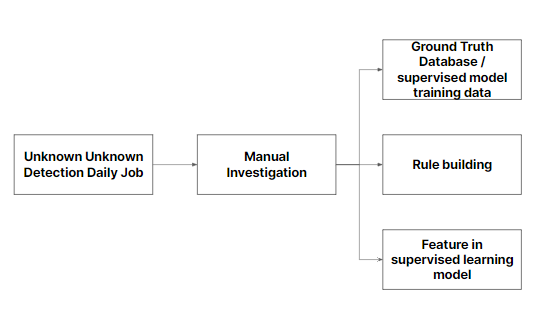
\includegraphics[width=0.5\textwidth]{vision_flowchart.PNG}
    \caption{Unknown Unknowns Detection Vision}
    \label{fig:vision_flowchart}
\end{figure}

\subsection{Hypotheses}\label{sec:hypotheses}
Our work is motivated by two central hypotheses:
\begin{enumerate}
    \item \textbf{Feature Volume Hypothesis: } We hypothesize that spoofers are unable to consistently mask all of the features we record. The odds are stacked against them: a single slip-up will give them away.

          $\newline$
          This relates to our earlier discussion on our vision for the impact of unknown unknowns detection on rules optimization. It's the centerpiece of this study and of strong interest to senior leadership.
    \item \textbf{Spoofing Scarcity Hypothesis: } We hypothesize that spoofed transactions are strongly underrepresented: their impact on transaction statistics is weak.

          $\newline$
          The practical implication of this hypothesis is that unsupervised learning (and in particular anomaly\ outlier detection) can be leveraged to extract spoofing-related unknown unknowns. Had we been interested in discovering signals related to a common transaction class, there would be no hope in this endeavour. It's interesting to note that spoofing scarcity is often brought up in the context of our supervised learning research, where it leads to undesireable class imbalance. In this respect, our research direction rehashes a common liability of fraud detection ML/ AI applications into an asset.
\end{enumerate}

\subsection{Objectives}\label{sec:Objectives}
In order to test our hypotheses (and leverage their validity in case they are found to hold), we set out to create an unknown unknowns discovery system based on unsupervised anomaly detection.

$\newline$
Our objective was to design and implement a model capable of identifying and explaining each of the following \textbf{three} anomaly types:
\begin{enumerate}
    \item \textbf{Marginal Distribution Anomalies}: out-of-distribution values.

          $\newline$
          Marginal distribution anomalies refer to outlier values found within samples from univariate distributions of individual features. They are the simplest of the three anomaly types we aim to detect. To illustrate, an example would be identifying high WiFi altitude values within an Ontario-based dataset (Ontario is flat).

    \item \textbf{Conditional Distribution Anomalies}: unusual combinations of values in different columns.

          $\newline$
          Conditional distribution anomalies refer to feature combinations that violate majority-class patterns. An example would be given by mismatches between highly correlated columns (e.g. the \texttt{ip\_country\_code} and \texttt{wifi\_country\_code}).

    \item \textbf{Representational Anomalies}: anomalies related to the representation of a record, rather than the value it denotes.

          $\newline$
          By \textit{representational anomalies} (a non-standard term) we refer to irregularities in the string representation of numeric data. Our current NDBS rule system conditions on the number of digits in lat/ lon records. We hypothesize that synthetic requests sent by spoofers can result in various unknown representational irregularities in the fields they mask. One of our primary objectives was to design a general algorithm capable of detecting them.
\end{enumerate}

Under our hypotheses, our historic transaction data will be rich in spoofing instances exemplifying these three anomaly types. The validity of the \textit{feature volume hypothesis} will result in the existence of spoofing transactions violating latent patterns. The validity of the \textit{spoofer scarcity hypothesis} will result in such transactions being a small minority. Consequently, when viewed alongside our extensive transaction records, they would constitute anomalies.

$\newline$
The successful implementation of an anomaly detector able to:
\begin{enumerate}
    \item flag these outlier transactions,
    \item attribute its decision to profound novel signals related to spoofing,
\end{enumerate}
would smiultaneously provide positive evidence for our hypotheses and yield a working unknown unknowns detector leveraging their validity for the advancement of the company's interests. Our objective is to develop such a system.

\subsection{Early Achievements}\label{sec:early_achievements}
Early versions of the model were applied to production data from the PLC and NDBS solutions. To be specific, we studied the PLC US7 complete history from 01/08/23 to 07/08/23 (301,377 transactions, 56 utilized features) and the NDBS BET99 ON \& Betano ON complete history from 01/11/23 to 15/11/23 (384,343 transactions, 277 utilized features).

$\newline$
The results quickly demonstrated potential. By inspecting the top transactions flagged by our system, we immediately spotted multiple interpretable anomalies. Identified signals included:
\begin{enumerate}
    \item Mismatches between the IP and WiFi geolocation sources.
          \begin{figure}[htbp]
              \centering
              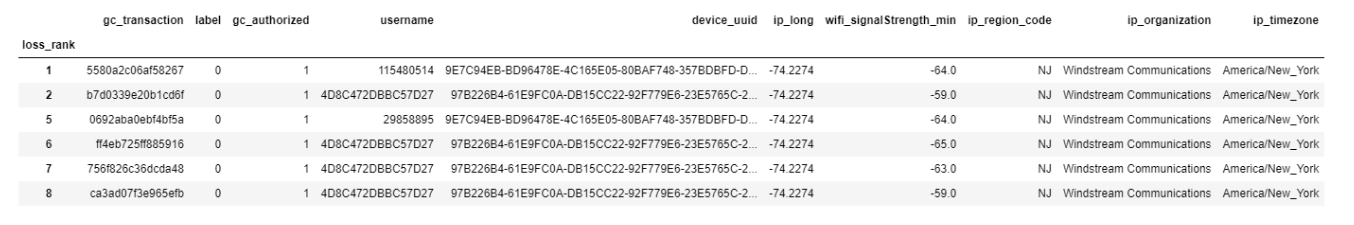
\includegraphics[width=1\textwidth]{ip_wifi_transactions.PNG}
              \caption{IP/WiFi Mismatches: Spoofing Colorado Transactions with NJ IPs}
              \label{fig:ip_wifi_transactions}
          \end{figure}

          \begin{figure}[htbp]
              \centering
              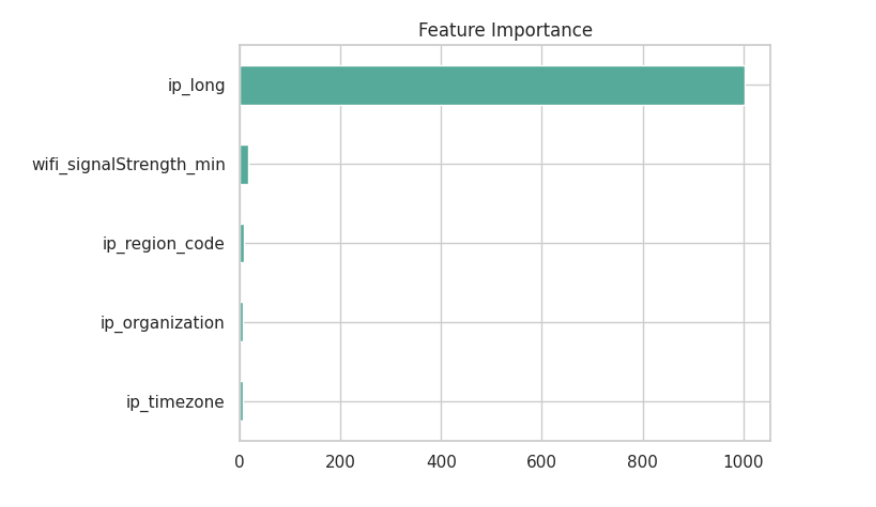
\includegraphics[width=0.7\textwidth]{ip_wifi_features.PNG}
              \caption{IP/WiFi Mismatches: Interpretation}
              \label{fig:ip_wifi_features}
          \end{figure}
    \item WiFi coordinate representation anomalies. Trailing zeros in the WiFi coordinates of transactions exhibiting IP/ WiFi mismatch. The WiFi was in Miami and the IP in Argnetina. The WiFi coordinates appear to have been masked.

          \begin{figure}[htbp]
              \centering
              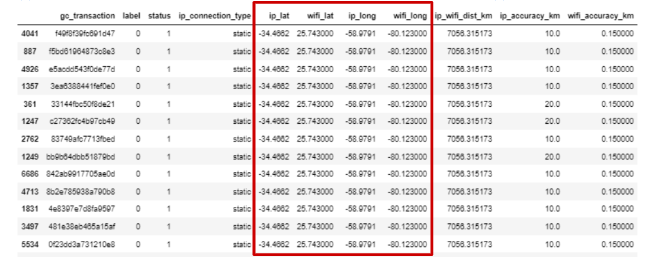
\includegraphics[width=0.7\textwidth]{repr_transactions.PNG}
              \caption{WiFi Coordinate Representational Anomalies: Transactions}
              \label{fig:repr_transactions}
          \end{figure}

          \begin{figure}[htbp]
              \centering
              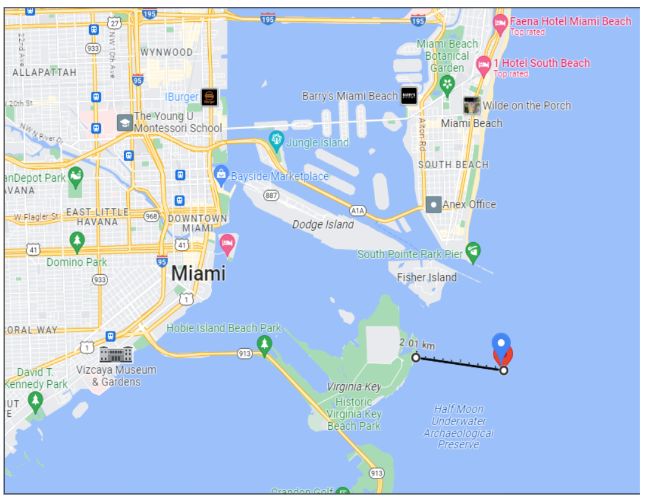
\includegraphics[width=0.7\textwidth]{repr_map.PNG}
              \caption{WiFi Coordinate Representational Anomalies: Map}
              \label{fig:repr_map}
          \end{figure}

          \begin{figure}[htbp]
              \centering
              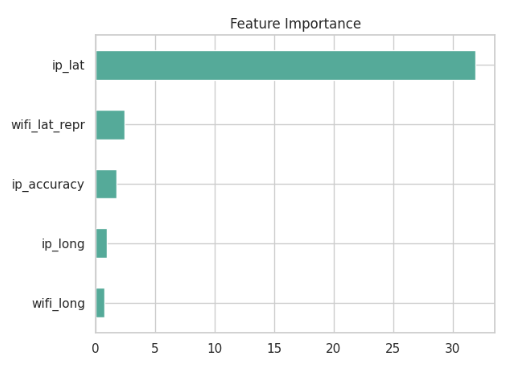
\includegraphics[width=0.7\textwidth]{repr_features.PNG}
              \caption{WiFi Coordinate Representational Anomalies: Interpretation}
              \label{fig:repr_features}
          \end{figure}
          \newpage
    \item WiFi access point irregularities: Multiple access points with identical signal properties.

          \begin{figure}[htbp]
              \centering
              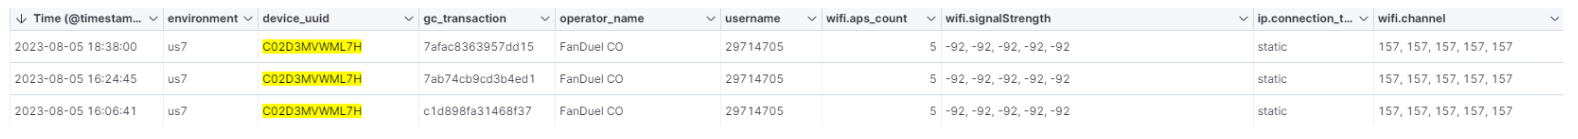
\includegraphics[width=1\textwidth]{wifi_aps.PNG}
              \caption{WiFi Access Point Spec Anomalies}
              \label{fig:wifi_aps}
          \end{figure}

    \item WiFi altitude irregularities: $\texttt{wifi\_altitude} > 3000\; \mathrm{m}$ in Ontario.

          \begin{figure}[htbp]
              \centering
              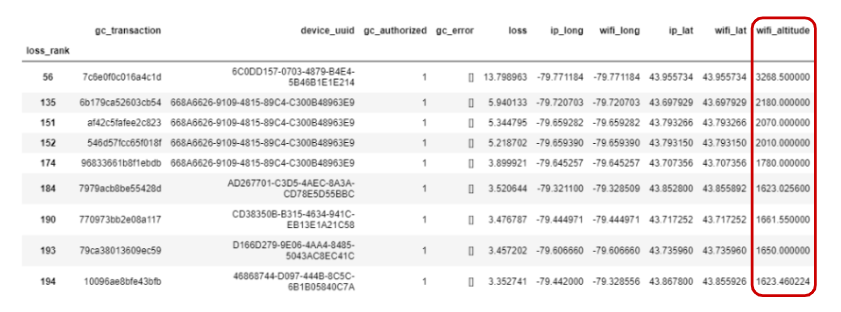
\includegraphics[width=1\textwidth]{altitudes.PNG}
              \caption{Altitude Anomalies}
              \label{fig:altitudes}
          \end{figure}
\end{enumerate}

$\newline$
Our findings instigated manual review aimed at determining whether we'd correctly identified instances of spoofing. Most of the flagged transactions were confirmed as such.

$\newline$
Notably, we identified twenty-four (24) high-risk transactions exhibitng significant mismatches between their IP and WiFi coordinates. Fifteen (15) of these were confirmed to be spoofing cases. This verdict sparked interest in further investigatation into the signal. The findings led to the discovery---and eventual blocking---of 4 distinct spoofer-operated devices. The transactions were added to the groundtruth dataset. This ultimately resulted in reevaluating a recent amendment to our rules system related to the treatment of IPs outside of the US/ Canada. The aforementioned developments are all stronlgy encouraging indicators that our proposed research direction is in alignment with our objectives:
\begin{enumerate}
    \item Our system was already able to identify a signal responsible for the actionable (blocking) identification of spoofers' devices.
    \item Our system was already able to contribute to the breadth of spoofing activity represented in the groundtruth dataset.
    \item Our system was already able to contribute to rules optimization.
\end{enumerate}
These achievements are in direct alignment with the objectives set out in the previous sections.

$\newline$
Among the spoofing cases, we also discovered anomalous transactions that did not strictly adhere to our current spoofing criteria. All of them were peculiar in immediatley identifiable ways. The reviewers' verdict was that they were the result of data collection error. This is still an encouraging development in two ways:
\begin{enumerate}
    \item It demonstrates the capacity of our system to flag interpretable signals not confined within our current understanding of the spoofing landscape.
    \item Unearthing unfamiliar data collection errors can help us identify liabilities in our data. By addressing these liabilities, we can improve the performance of our data science efforts at large.
\end{enumerate}

\section{Solution}
Our anomaly detector is based on the autoencoder architecture. We detect represetnational anomalies by leveraging stacked attention encoders (BERT) and having the autoencoder reconstruct the resulting embedding means in a simple transfer learning procedure.

\subsubsection{\texttt{TextEncoder}}
Our \texttt{TextEncoder} network is designed to encode text data. It's an implementation of BERT \cite{BERT}. Even though---in principle---it could be used to extract meaningful patterns from natural language excerpts, the application we have in mind relates to the identification of irregularities in the string representation of numerical records. Our objective is to produce an embedding that clusters the records into classes so that all regular records group together and all irregularity types correspond to unique and well-separated clusters.
\begin{figure}[htbp]
    \centering
    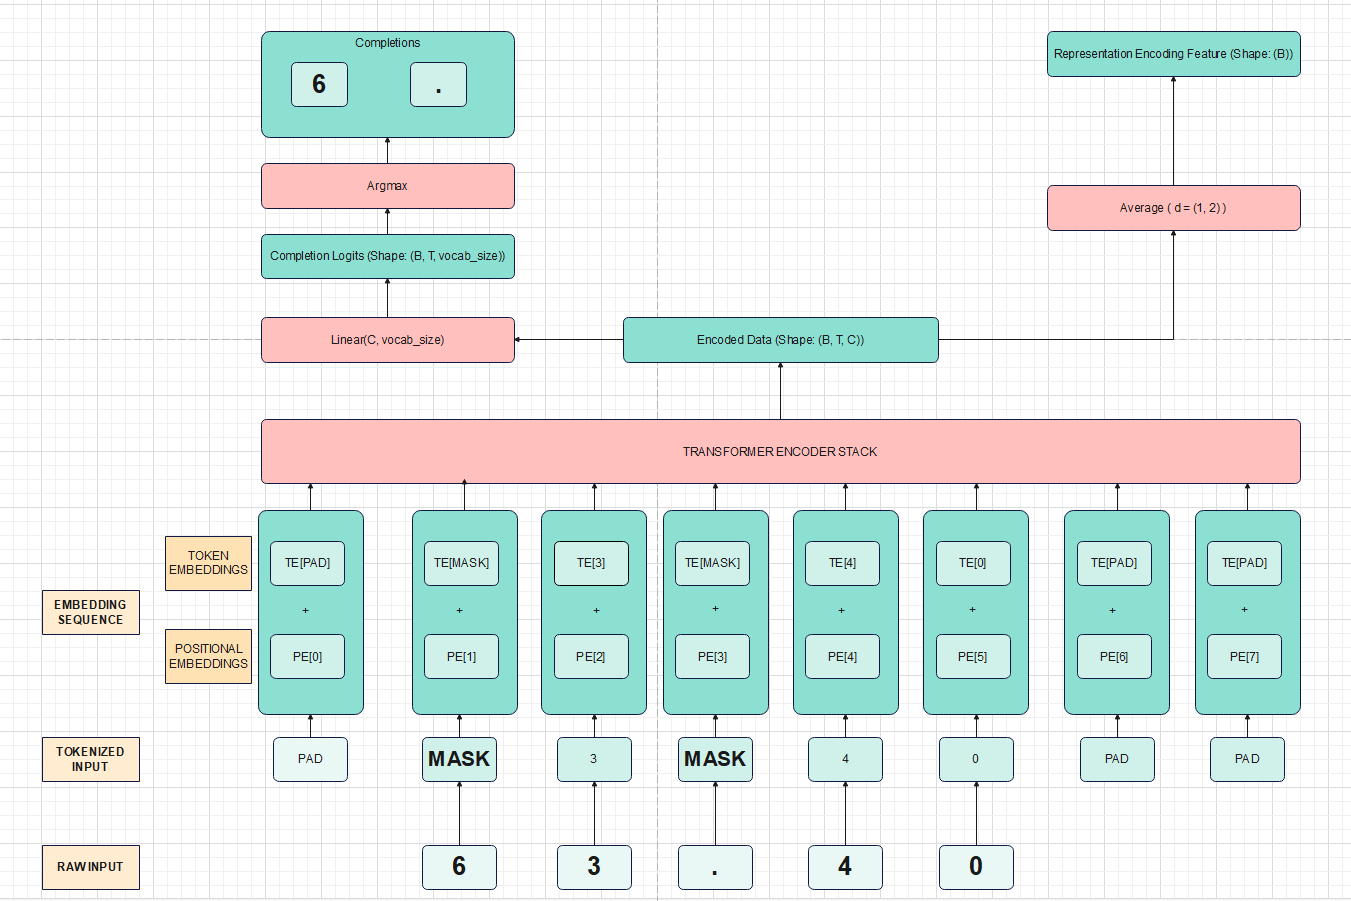
\includegraphics[width=1\textwidth]{bert_graph.PNG}
    \caption{\texttt{TextEncoder} Architecture}
    \label{fig:bert_graph}
\end{figure}
We train small (~3000 parameters) character-level models for each numeric column of interest. This allows us to map entries of numeric columns to tensors of shape:
\begin{equation}
    \texttt{shape} = (T, C).
\end{equation}
Here, $T$ is the max string size accepted by the BERT model and $C$ is the token embedding dimension. Averaging the entries of these tensors, we are able to express the representation of any given numeric column through a single derived feature. These features are added to the dataset that will be eventually parsed by the autoencoder.

$\newline$
The network is not directly trained with anomaly detection in mind. Instead, we apply the MLM pretraining procedure from \cite{BERT}. During training, fifteen percent of incoming tokens are selected---at random---for modification. Ten percent of these are randomly resampled. Eighty percent are replaced with a designated \texttt{mask\_token} concealing their content. The remaining ten eprcent are left unaltered. The model is trained to unmask the masked tokens (complete the text). In doing so it's forced to seek and leverage latent patterns in the token sequenes. This results in the discovery of an effective represetnation reflecting these patterns. We are not interested in token completions. We merely use this process to gain access to the encoding that facilitates them.

$\newline$
The process is illustrated in \figref{fig:bert_graph}. The figure depcits the process of extracting the representation encoding of the number $63.40$. The first and third characters are masked and the resulting token sequence is passed through the network (stacked bidirectional multi-head attention). The resulting encoding is leveraged for text completion. The encoding is then averaged and the representation feature is extracted.

\subsubsection{\texttt{TransactionAnomalyDetector}}
Our \texttt{TransactionAnomalyDetector} network is the centerpiece of this project. It's a feedforward autoencoder designed to support both continuous and categorical features. \figref{fig:ae_graph_full} illustrates the architecture.

\begin{figure}[htbp]
    \centering
    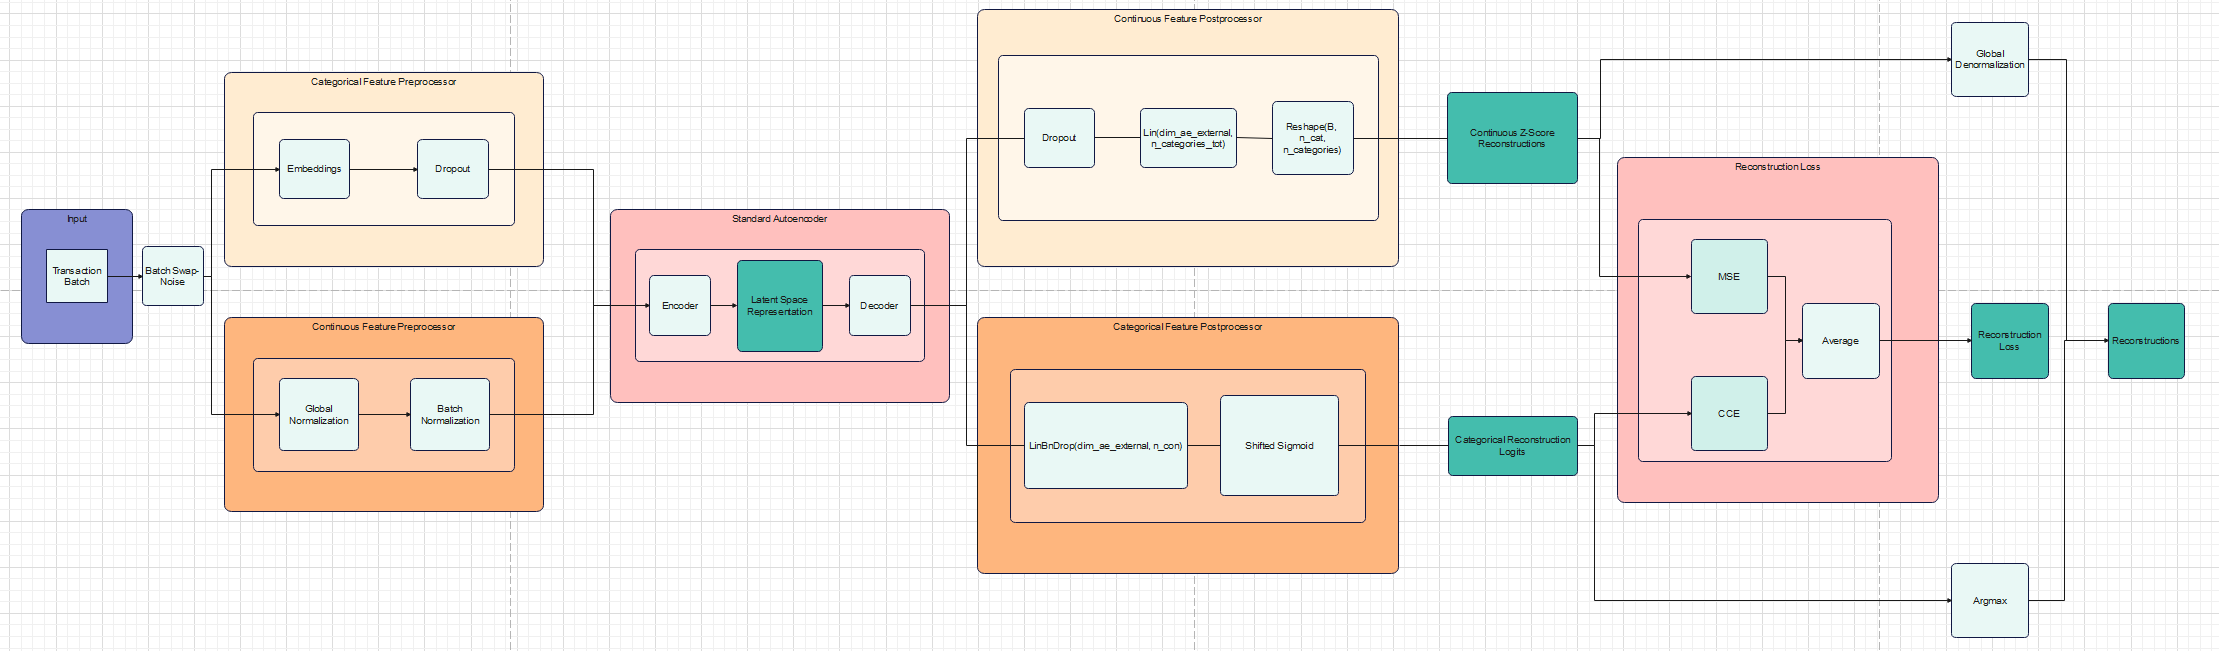
\includegraphics[width=1\textwidth]{ae_graph_full.PNG}
    \caption{\texttt{TransactionAnomalyDetector} Architecture}
    \label{fig:ae_graph_full}
\end{figure}
The model works with tabular data. It expects a certain set of continuous and categorical features. Input records are expected to offer all of these.

$\newline$
The first layer in the network is an implementation of \texttt{swap\_noise} operating at the batch-level. Like dropout \cite{Dropout}, this only operates during training. Its function is to resample a fixed proportion (\texttt{swap\_rate}) of batch entries from their respective columns. This is intended to force the autoencoder to identify latent intra-feature relationships. The addition of this layer upgrades our model from a simple autoencoder to a \textit{denoising autoencoder}. Without the added noise, we run the risk of having individual features play dominant roles in their own reconstructions. This would go against our intention of capturing hidden unknown patterns.

$\newline$
Continuous features and categorical features are preprocessed differently. At the start of the training process, the model collects global population statistics (min, max, mean and standard deviation) for each continuous feature. It uses these statistics to map incoming values to z-score space. We refer to the corresponding normalization procedure as \textit{global normalization}. Responsible for it is the first component of the \textit{continuous feature preprocessor} (\figref{fig:ae_graph_full}). The autoencoder is trained to receive and reconstruct z-scores. Once this is achieved, global normalization can be undone using the recorded global population statistics once more. The second component of the continuous feature preprocessor is a batch normalization layer \cite{BatchNorm}. This is intended to scale and center the itra-batch z-score values so as to expidate network convergence. Categorical features are passed through learned embedding layers and the resulting embeddings are filtered through a dropout layer whose rate is hardcoded to:
\begin{equation}\nonumber
    \texttt{\_dropout\_rate\_cat\_decoder} = 0.1.
\end{equation}
This is independent of the \texttt{dropout\_rate} used in the rest of the network.

$\newline$
The preprocessed inputs are then passed through a standard feedforward autoencoder.
\begin{figure}[htbp]
    \centering
    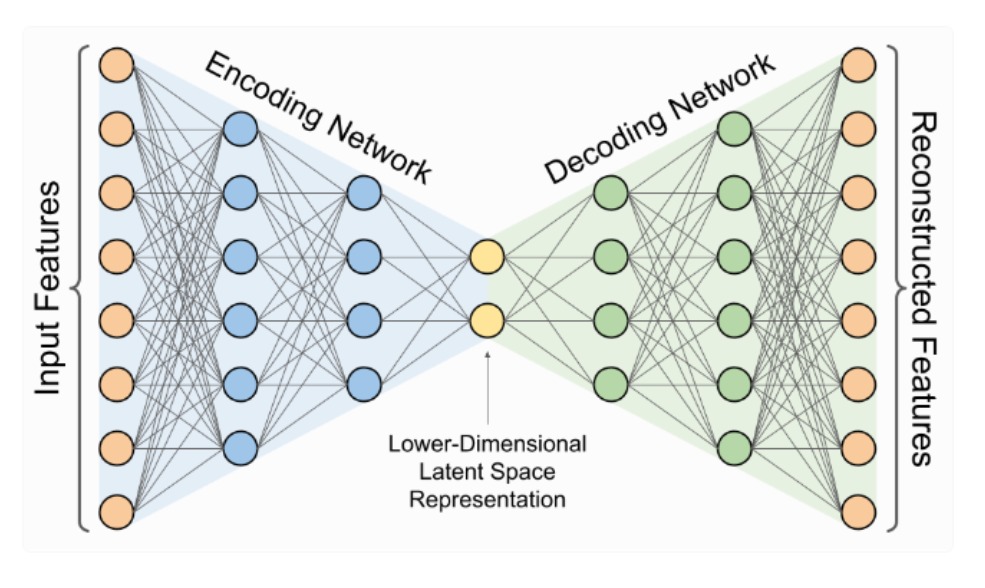
\includegraphics[width=1\textwidth]{standard_autoencoder.PNG}
    \caption{Standard Feedforward Autoencoder}
    \label{fig:standard_autoencoder}
\end{figure}
This consists of an encoder and a decoder. The encoder compresses the original inputs. The decoder reconstructs the original inputs from their compressed form. To achieve this, the standard autoencoder has to learn latent patterns in the data. When these patterns are disturbed, reconstructions fail. Reconstruction failure can be leveraged for anomaly detection. To encode and decode the data, the standard autoencoder uses stacked linear layers with dropout and batch normalization (\texttt{LinBnDrop}). The standard autoencoder receives an input signal of higher dimension than the concatenated continuous features and categorical token embeddings (\textit{preprocessed input}). To achieve this, the preprocessed input is passed through a linear layer of configurable shape whose output matches the size of the first encoder layer. The layer sizes of the encoder and the decoder \texttt{MLPs} are mirrored (\textit{hourglass architecture}) as in \figref{fig:standard_autoencoder}.

$\newline$
Once the decoded output has been obtained, it needs to be parsed to form the feature reconstructions. This is the job of the \textit{continuous feature postprocessor} and the \textit{categorical feature postprocessor} modules. It's crucial to note that the decoder's output size does not directly match the number of underlying features (sum of continuous features and categorical embedding dimensions). Instead, it constitutes a reconstruction internal to the model: one that mixes signals from various features together. Both the continuous and the categorical postprocessors cast this signal to the respective necessary dimension. To do so, they each leverage a linear layer. The former filters the output of this layer through parallel sigmoid functions (one for each feature) with horizontal asymptotes determined using the recorded global population statistics:
\begin{align}
    \texttt{sigmoid\_min} = \frac{\texttt{min}-\mu}{\sigma},\nonumber \\
    \texttt{sigmoid\_max} = \frac{\texttt{max}-\mu}{\sigma}.\nonumber
\end{align}
Here, $\mu$ and $\sigma$ denote the respective continuous feature's mean and standard deviation, whereas \texttt{sigmoid\_min} and \texttt{sigmoid\_max} denote the corresponding sigmoid function's asymptotes:
\begin{equation}\nonumber
    \texttt{shifted\_sigmoid} = \texttt{sigmoid\_min} + \left(\texttt{sigmoid\_max} - \texttt{sigmoid\_min}\right)\cdot\texttt{standard\_sigmoid}.
\end{equation}
The categorical feature preprocessor casts the decoder's output to a vector with length equal to the sum of the embedding dimensions. This tensor is then reshaped to obtain the logits encoding the model's estimates of the respective multinoulli distributions.

$\newline$
Once the reconstructed z-scores and logits have been obtained, their deviation from the original record is measured by the \textit{reconstruction loss} module. This applies MSE to the z-scores and CCE to the logits. The record's reconstruction loss is obtained by averaging the individual feature losses with equal weights.

$\newline$
Anomalies are flagged by learning a reconstruction loss threshold using a configurable quantile. The latter is determined by passing a \texttt{contamination} parameter:
\begin{equation}\nonumber
    \texttt{reconstruction\_loss\_quantile} = 1 - \texttt{contamination}.
\end{equation}
\subsubsection{Anomaly Interpretation \& Signal Identification}
Once the \texttt{TransactionAnomalyDetector} has flagged an anomalous record, it's required to communicate its decision process. This is a critical component of our system: it constitutes the process by which novel spoofing signals are to be discovered. This is achieved by applying the method in \cite{AeInterp}.

$\newline$
The method is based on Kernel SHAP\cite{SHAP} feature attributions. Shapely values are estimated using local linear regression on a dataset of perturbations of the anomaly (transaction) to be explained. This produces feature attribution scores explaining the reconstruction logic for the features that most dominantly contributed to the total reconstruction loss. In layman's terms, we ask the model to explain its logic where it failed to produce faithful reconstructions. The idea is simple: reconstruction failure correlates to violation of latent patterns discovered during training. A successful expression of the erroenous reconstruction logic should capture these patterns and the way in which they were violated. This is precisely what's required to identify the relevant spoofing signal.

$\newline$
The output of the process can be communicated using plots such as the one in figure \figref{fig:attr_example}. The whole plot is dedicated to explain a single anomalous transaction. Rows correspond to the most dominant contributors to the total reconstruction loss. Columns correspond to all available features. Color intensity encodes absolute feature attribution scores (Kernel SHAP coefficients). Green indicates that the feature corresponding to the relevant column helped offset the erroenous reconstruction of the feature corresponding to the relevant row. Red indicates the opposite: a contribution to the anomaly.
\begin{figure}[htbp]
    \centering
    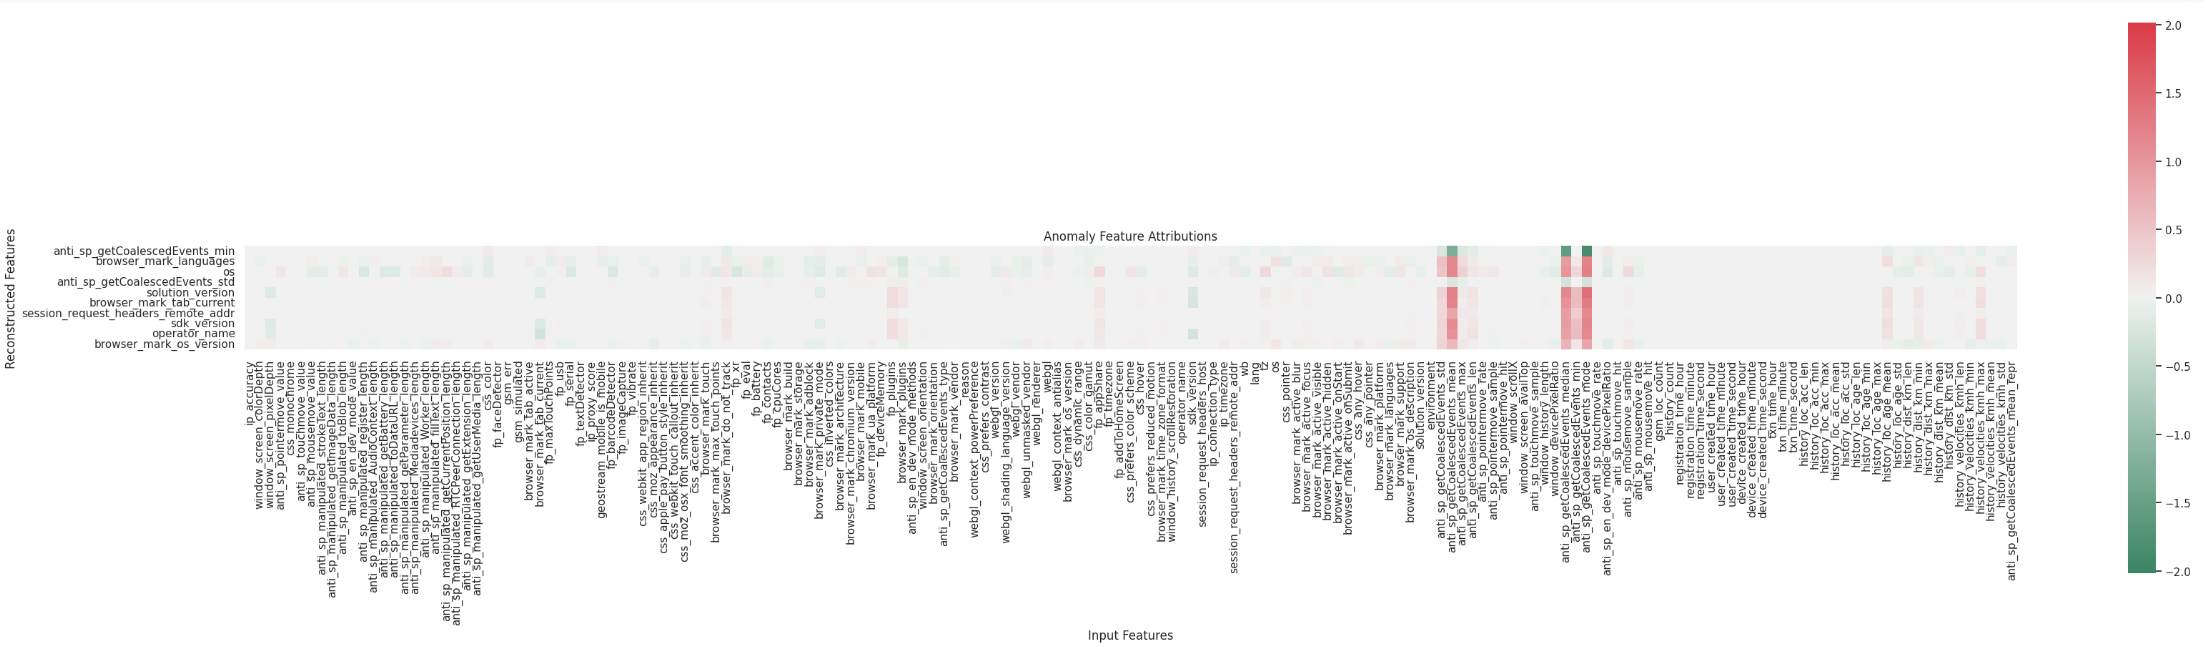
\includegraphics[width=1\textwidth]{attr_example.png}
    \caption{Anomaly Interpretation Plot}
    \label{fig:attr_example}
\end{figure}
\subsubsection{Integration: Anomaly Detection Pipeline}
We now provide an overview of all the components comprising our anomaly detection process and illustrate how it works to identify the three anomaly types we set out to discover. Note that this does not cover the full extent of our process: it omits our work on data cleaning/ preprocessing and geographical segmentation. These are the subject of section \ref{sec:training_clustering}. Our objective here is merely to illustrate the functionality of our model. In the context of the diagrams that follow, anomalies are indicated using red frames. Normal instances are indicated using green frames.

$\newline$
Overall, our process can be summarized by the following flowchart:
\begin{figure}[H]
    \centering
    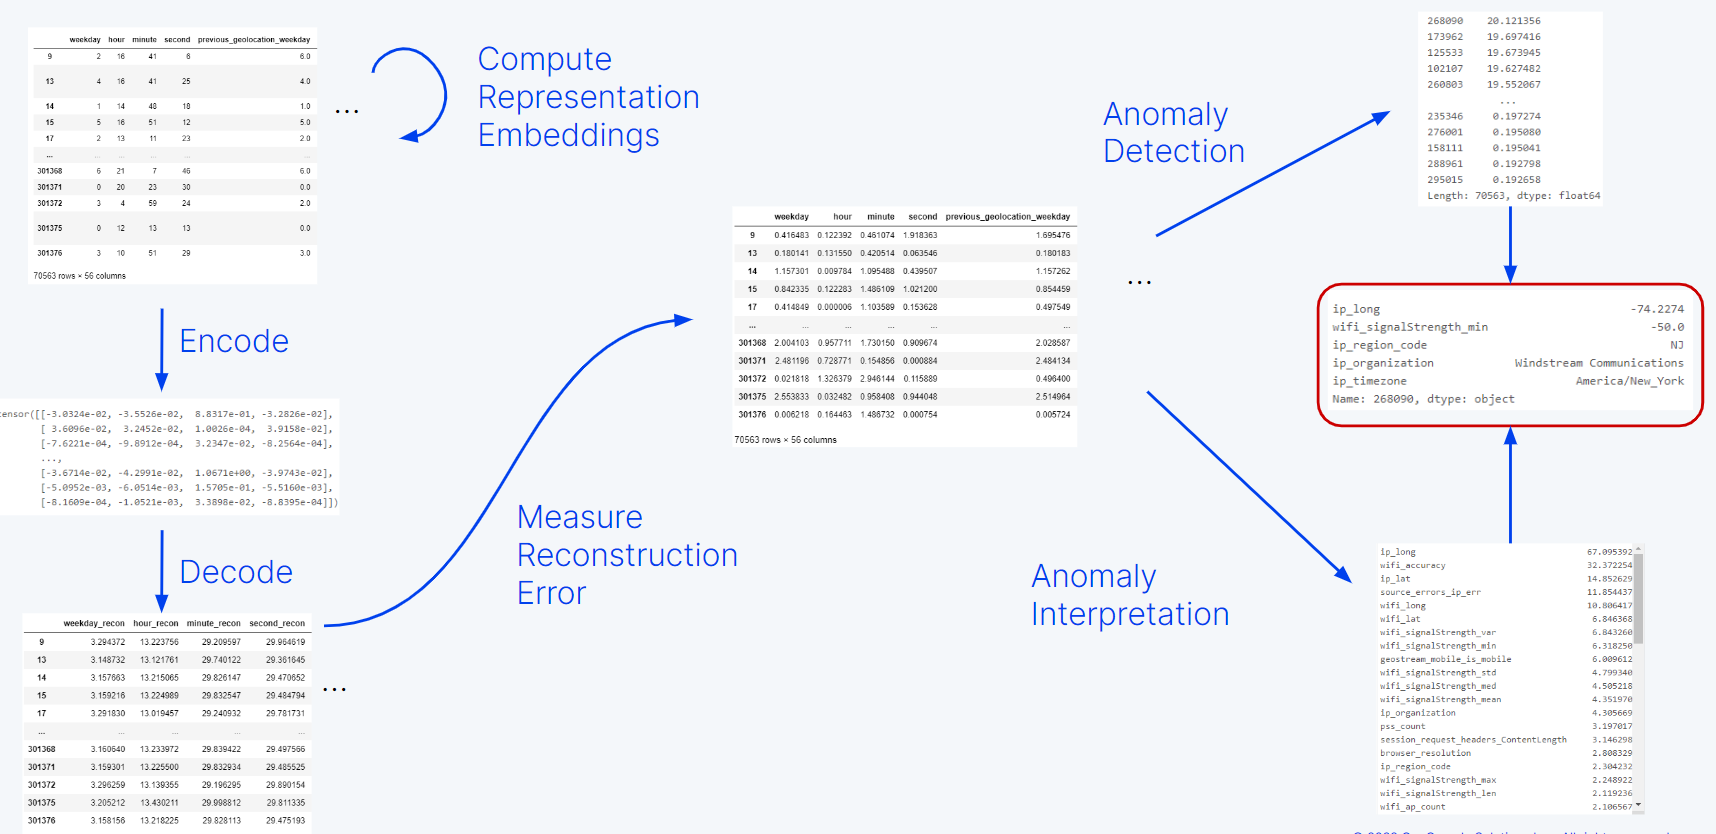
\includegraphics[width=1\textwidth]{process_flowchart.PNG}
    \caption{Anomaly Detection Process Flowchart}
    \label{fig:process_flowchart}
\end{figure}
The model accepts a dataframe of ~70000 transactions. These are immediately enriched with representation encodings. The enriched transactions are compressed (encoded) and the compressions are fed into the decoder module. The reconstruction loss is measured and both transactions and features are ranked by it. This leads to the isolation of a single record and ten features exhibitng the WiFi/ IP mismatch signal discussed in section \ref{sec:early_achievements}.

$\newline$
To illustrate how the model detects each of the three anomaly types introduced in section \ref{sec:Objectives}, we work with synthetic data. Our synthetic dataset contains four features:
\begin{enumerate}
    \item \texttt{wifi\_lat} (continuous),
    \item \texttt{wifi\_lon} (continuous),
    \item \texttt{n\_access\_points} (categorical),
    \item \texttt{triangulation\_accuracy} (categorical).
\end{enumerate}
The coordinates were randomly sampled around New York City. The number of access points was sampled uniformly randomly:
\begin{equation}\nonumber
    \texttt{n\_access\_points} \sim\mathcal{U}\left\{2, 3, 4, 5, 6\right\}.
\end{equation}
The triangulation accuracy was determined from the number of access points uisng the map:
\begin{equation}\nonumber
    \texttt{triangulation\_accuracy} = \textit{accuracy\_map}\left(\texttt{n\_access\_points}\right),
\end{equation}
where:
\begin{equation}\nonumber
    \textit{accuracy\_map} =
    \begin{cases}
        2 & \mapsto \texttt{very low}   \\
        3 & \mapsto \texttt{low}        \\
        4 & \mapsto \texttt{medium}     \\
        5 & \mapsto \texttt{high}       \\
        6 & \mapsto \texttt{very high}.
    \end{cases}
\end{equation}

$\newline$
The flowchart in \figref{fig:marg_flowchart} exhibits the detection of a marginal distribution anomaly: two records have unusual coordinates.
\begin{figure}[htbp]
    \centering
    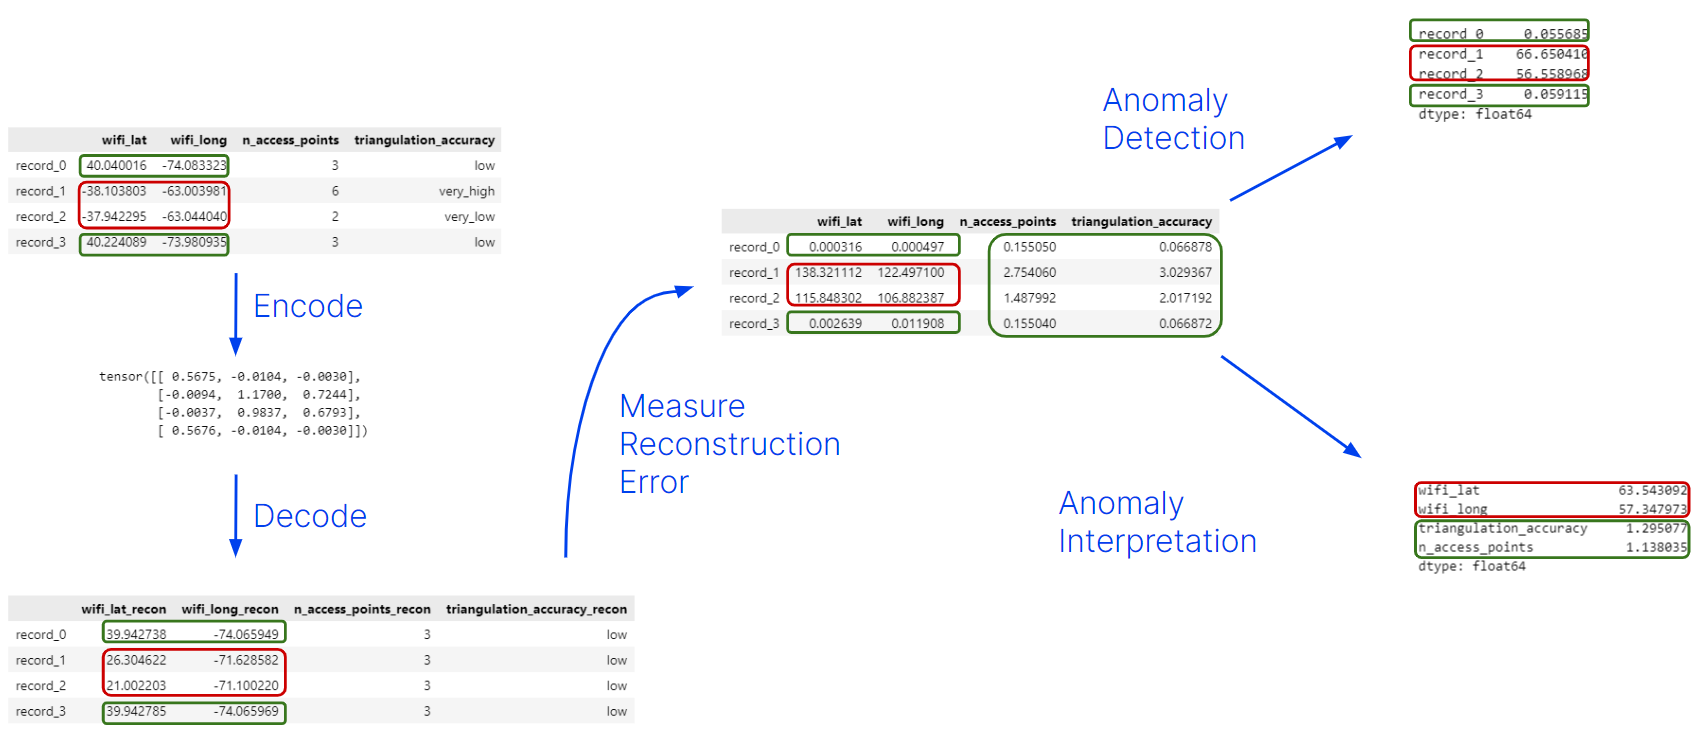
\includegraphics[width=1\textwidth]{marg_flowchart.PNG}
    \caption{Marginal Anomaly Detection Flowchart}
    \label{fig:marg_flowchart}
\end{figure}

$\newline$
The flowchart in \figref{fig:cond_flowchart} exhibits the detection of a conditional distribution anomaly: two records violate the relationship between the \texttt{n\_access\_points} and \texttt{triangulation\_accuracy} columns.
\begin{figure}[htbp]
    \centering
    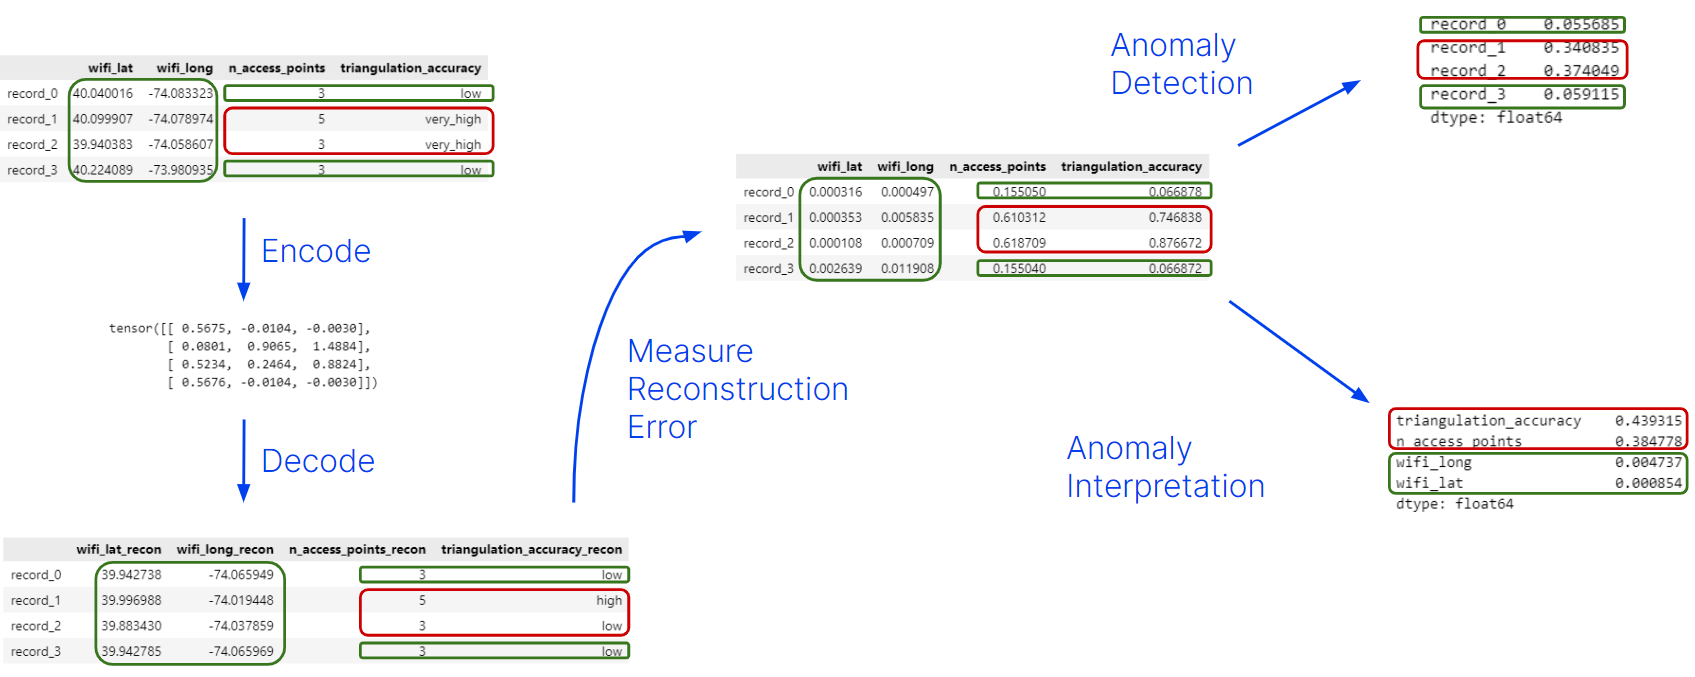
\includegraphics[width=1\textwidth]{cond_flowchart.PNG}
    \caption{Conditional Anomaly Detection Flowchart}
    \label{fig:cond_flowchart}
\end{figure}

$\newline$
The flowchart in \figref{fig:repr_flowchart} exhibits the detection of a representational anomaly: multiple records have trailing zeros in their coordinate fields.
\begin{figure}[htbp]
    \centering
    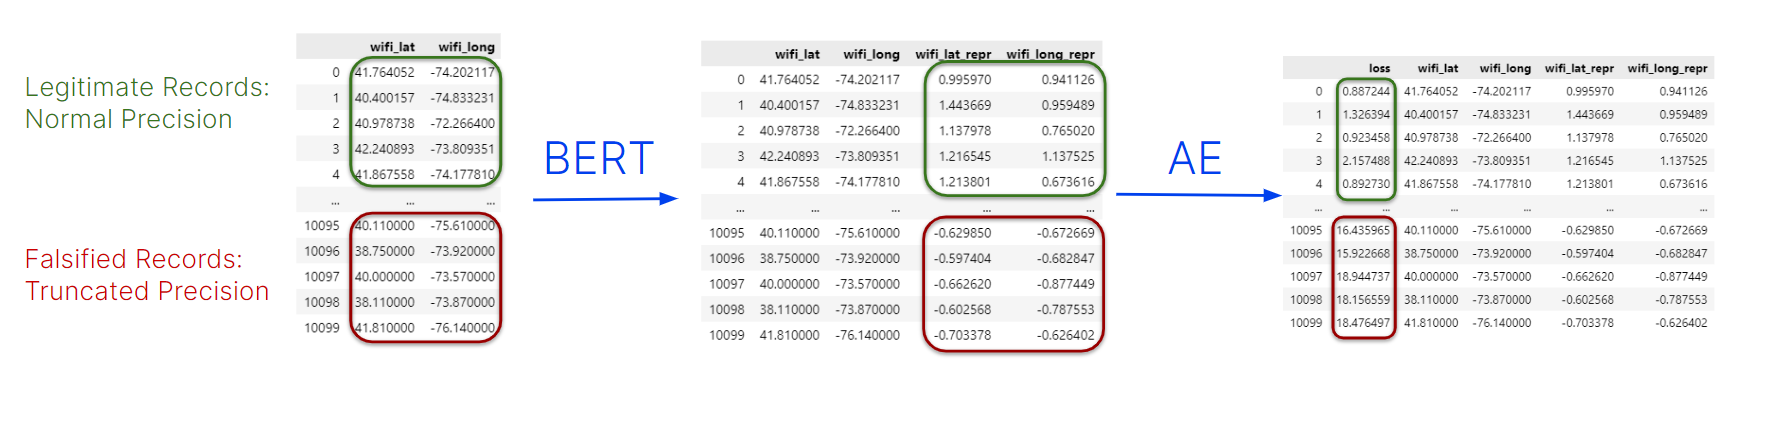
\includegraphics[width=1\textwidth]{repr_flowchart.PNG}
    \caption{Representational Anomaly Detection Flowchart}
    \label{fig:repr_flowchart}
\end{figure}

\newpage
\section{API Reference}
% dir
\subsection{\texttt{clustering}}
This directory contains tools to cluster transactions based on their location.

$\newline$
The classes provided are:
\begin{enumerate}
    \item \texttt{clustering}:
          \begin{enumerate}
              \item \texttt{ClusterIdentifier}.
          \end{enumerate}
\end{enumerate}

\subsubsubsection{Class \texttt{ClusterIdentifier}}

\begin{description}
    \item[Description:] An interface for grouping labeled geolocation transactions in nearest neighbour (NN) clusters. The \texttt{ClusterIdentifier} is trained on a fixed collection of transactions. It partitions this collection into NN clusters and stores the results internally. It exposes cluster composition statistics to the user, who can then retrieve the desired cluster using an internal indexing system. Input transactions ought to be stored in a geopandas geodataframe including a \texttt{label} column. In practice this should either be set to \texttt{NOT gc\_authorized}, pseudolabels derived from \texttt{gc\_error} criteria or the manual review labels on \texttt{groundtruth}. Class balance statistics derived from the labels are meant to be used as a criterion for cluster selection.
    \item[Constructor Parameters:] \texttt{None}.
    \item[Attributes:] \texttt{df\_cluster\_stats (pd.DataFrame)}: A dataframe exposing cluster composition statistics (cluster index, distance to centerpoint statistics, class balance).
\end{description}

\subparagraph{Method \texttt{get\_cluster()}}

\begin{quote}
    \begin{description}
        \item[Description:] Retrive the desired cluster by providing its index. The latter can be found by inspecting \texttt{df\_cluster\_stats}.
        \item[Parameters:] \texttt{cluster\_idx (int)}: Index of desired cluster (found by inspecting \texttt{df\_cluster\_stats}).
        \item[Returns:] \texttt{(gpd.GeoDataFrame)} The desired cluster represented as a geodataframe.
    \end{description}
\end{quote}

\subparagraph{Method \texttt{fit()}}
\begin{quote}
    \begin{description}
        \item[Description:] Partition a collection of geolocation transactions in NN clusters and store results in internal state.
        \item[Parameters:] $\newline$
            \begin{enumerate}
                \item \texttt{gdf\_transactions (gpd.GeoDataFrame)}: Transaction collection. This is required to have a binary \texttt{label} column as discussed in the class description.
                \item \texttt{n\_nbrs (int)}: Number of nearest neighbours.
                \item \texttt{crs (str)}: Local projected coordinate system for geodesic distance computation.
                \item \texttt{gdf\_centers (Optional[gpd.GeoDataFrame])}: Transactions to use as cluster centers. Defaults to transactions in the positive class.
            \end{enumerate}
        \item[Returns:] \texttt{None}
    \end{description}
\end{quote}

\newpage
\begin{lstlisting}[language=Python, caption=\texttt{ClusterIdentifier} Demo]

    # Initialize the cluster identifier.

    cluster_identifier = ClusterIdentifier()

    # Train it on a gdf (gdf_local_transactions) containing a collection of geolocation transactions. Center the clusters at transactions carrying positive pseudolabels.

    cluster_identifier.fit(
        gdf_transactions=gdf_transactions,
        n_nbrs=100,
        crs='EPSG:4326',
        gdf_centers=gdf_local_transactions[gdf_local_transactions['label'] == 1]
        )

    # Display the identified clusters so as to decide which cluster to work with.

    display(cluster_identifier.df_cluster_stats)

    # Determine the relevant cluster index by inspecting df_cluster_stats.

    cluster_idx = 10

    # Access the desired cluster.

    gdf_cluster = cluster_identifier.get_cluster(cluster_idx=cluster_idx)
\end{lstlisting}

% dir
\subsection{\texttt{models}}
This is the core directory of the project. It contains all the functionality related to our models.

$\newline$
The classes provided are:
\begin{enumerate}
    \item \texttt{tools}: auxiliary tools used to train and operate our NN models:
          \begin{enumerate}
              \item \texttt{tokenization}:
                    \begin{enumerate}
                        \item \texttt{Tokenizer},
                    \end{enumerate}
              \item Training
                    \begin{enumerate}
                        \item \texttt{early\_stopping}:
                              \begin{enumerate}
                                  \item \texttt{EarlyStopperBase},
                                  \item \texttt{StandardStopper},
                                  \item \texttt{MonotoneStopper},
                              \end{enumerate}
                        \item \texttt{TrainerBase},
                    \end{enumerate}
          \end{enumerate}
    \item \texttt{layers}:
          \begin{enumerate}
              \item \texttt{BatchSwapNoise},
              \item \texttt{ContinuousFeatureNormalizer},
              \item \texttt{LinBnDrop},
              \item \texttt{MaskedCCELoss},
              \item \texttt{ReconstructionLoss},
              \item \texttt{ShiftedSigmoid},
              \item \texttt{TransformerEncoder},
          \end{enumerate}
    \item \texttt{text\_encoder}:
          \begin{enumerate}
              \item \texttt{TextEncoder},
          \end{enumerate}
    \item \texttt{autoencoder}:
          \begin{enumerate}
              \item \texttt{TransactionAnomalyDetector},
          \end{enumerate}
\end{enumerate}

\subsubsection{\texttt{tools}}
Within \texttt{transaction\_anomaly\_detection.models.tools} live auxiliary tools supporting the operation and training of our neural network models. These include a \texttt{Tokenizer} class and tools required for neural network training: the \texttt{TrainerBase} abstract base class and different kinds of early stopping tools for regularization.

\subsubsubsection{Class \texttt{Tokenizer}}

\begin{description}
    \item[Description:] The \texttt{Tokenizer} offers a simple API to encode a given collection of tokens---or sequences thereof---into integers. Once token sequences have been encoded, they can be decoded back to their original form. By fixing a body of text and letting the tokens be the alphabet, the \texttt{Tokenizer} acts as a character-level tokenization tool for simple NLP tasks.
    \item[Constructor Parameters:] $\newline$
        \begin{enumerate}
            \item \texttt{ls\_tokens (List[str])}: The set of regular tokens handled by the \texttt{Tokenizer} (e.g. the alphabet---iuncluding punctuation characters---in a character-level NLP application). This does not include special tokens for padding, handling unknowns and masking.
            \item \texttt{pad\_token (Optional[str])}: Special token used for padding. This is needed to increase the size of short sequences to appropriate lengths.
            \item \texttt{unk\_token (Optional[str])}: Special token representing an element absent from the \texttt{ls\_tokens}.
            \item \texttt{mask\_token (Optional[str])}: Special token used for masking. Regular tokens are replaced with the \texttt{mask\_token} to signify that their value has been hidden.
        \end{enumerate}
    \item[Attributes:] $\newline$
        \begin{enumerate}
            \item \texttt{vocabulary (Set[str])}: The set of all legitimate tokens: both regular and special. All sequences handled by the \texttt{Tokenizer} are valued in this set.
            \item \texttt{pad\_token (Optional[str])}: See the corresponding constructor parameter.
            \item \texttt{pad\_token\_encoding (Optional[int])}: The integer encoding of the \texttt{pad\_token}.
            \item \texttt{unk\_token (Optional[str])}: See the corresponding constructor parameter.
            \item \texttt{unk\_token\_encoding (Optional[int])}: The integer encoding of the \texttt{unk\_token}.
            \item \texttt{mask\_token (Optional[str])}: See the corresponding constructor parameter.
            \item \texttt{mask\_token\_encoding (Optional[int])}: The integer encoding of the \texttt{mask\_token},
            \item \texttt{regular\_token\_encodings (Set[int])}: The set of integer encodings of all regular tokens in the vocabulary.
        \end{enumerate}
\end{description}

\subparagraph{Method \texttt{pad()}}
\begin{quote}
    \begin{description}
        \item[Description:] Insert a prescribed amount of \texttt{pad\_tokens} on the left/ right of the input sequence.
        \item[Parameters:] $\newline$
            \begin{enumerate}
                \item \texttt{sequence (List[str])}: The token sequence to be padded.
                \item \texttt{pad\_left (Optional[int] = 0)}: Number of \texttt{pad\_tokens} to insert on the left.
                \item \texttt{pad\_right (Optional[int] = 0)}: Number of \texttt{pad\_tokens} to insert on the right.
            \end{enumerate}
        \item[Returns:] (List[str]) The padded token sequence.
    \end{description}
\end{quote}

\subparagraph{Method \texttt{encode()}} Map a token/ sequence of tokens to an integer/ sequence of integers.
\begin{quote}
    \begin{description}
        \item[Description:]
        \item[Parameters:] \texttt{token\_or\_ls\_tokens (str or List[str])}: The token/ token sequence to be encoded.
        \item[Returns:] \texttt{int or List[int]} The integer/ sequence of integers encoding th einput.
    \end{description}
\end{quote}

\subparagraph{Method \texttt{decode()}}
\begin{quote}
    \begin{description}
        \item[Description:] Map an encoded token/ sequence of encoded tokens to the original token/ token sequence that the input encodes.
        \item[Parameters:] $\newline$
            \begin{enumerate}
                \item \texttt{encoded\_token\_or\_ls\_encoded\_tokens (int or List[int])}: The integer sequence to be decoded.
            \end{enumerate}
        \item[Returns:] \texttt{str or List[str]}: The decoded token/ token sequence represented by the input.
    \end{description}
\end{quote}

\subparagraph{Method \texttt{str\_to\_ls\_tokens()}}
\begin{quote}
    \begin{description}
        \item[Description:] Character level string tokenization.
        \item[Parameters:] \texttt{str\_input: str}: The string to be tokenized.
        \item[Returns:] \texttt{(List[str])} The corresponding token sequence. This agrees with the list of characters comprising the input, excpet when they are not part of the \texttt{Tokenizer's} vocabulary.
    \end{description}
\end{quote}

\subparagraph{Method \texttt{ls\_tokens\_to\_str()}}
\begin{quote}
    \begin{description}
        \item[Description:] Join a sequence of tokens into a string, separating adjacent tokens by space characters.
        \item[Parameters:] \texttt{ls\_tokens (List[str])}: The token sequence to be joined
        \item[Returns:] \texttt{(str)} The joined token sequence.
    \end{description}
\end{quote}

\subsubsubsection{Abstract Class \texttt{EarlyStopperBase}}

\begin{description}
    \item[Description:] Abstract base class for early stopping tools. \texttt{EarlyStopperBase} implements only the core functionality required for early stopping, leaving the particular stopping criteria to be implemented in subclasses.
    \item[Constructor Parameters:] \texttt{max\_n\_epochs (int)}: Maximum number of training epochs.
    \item[Attributes:] $\newline$
        \begin{enumerate}
            \item \texttt{max\_n\_epochs (int)}: See the corresponding constructor parameter.
            \item \texttt{n\_epochs\_ellapsed (int)}: Number of training epochs completed thus far.
            \item \texttt{stop (bool)}: \texttt{True} iff the stopping condition has been satisfied.
            \item \texttt{best\_epoch (int)}: The number of the epoch when the monitored metric ahchieved its best value thus far.
            \item \texttt{best\_metric (int)}: Best value achieved for the monitored metric.
            \item \texttt{best\_model (nn.Module)}: The model state corresponding to the best metric.
        \end{enumerate}
\end{description}

\subparagraph{Method \texttt{update()}}
\begin{quote}
    \begin{description}
        \item[Description:] Update the \texttt{EarlyStopper's} internal state after changes to the monitored metric and model state. In practice, this method is to be called once at the end of each epoch.
        \item[Parameters:] $\newline$
            \begin{enumerate}
                \item \texttt{metric (float)}: The latest value of the monitored metric.
                \item \texttt{model (nn.Module)}: The latest model state.
            \end{enumerate}
        \item[Returns:] \texttt{None}
    \end{description}
\end{quote}
\subparagraph{Abstract Method \texttt{update\_stop\_state()}}

\begin{quote}
    \begin{description}
        \item[Description:] Decide if the stopping condition has been met and update internal state accordingly.
        \item[Parameters:] \texttt{None}
        \item[Returns:] \texttt{None}
    \end{description}
\end{quote}

\subparagraph{Abstract Class Method \texttt{stopping\_condition\_met()}}
\begin{quote}
    \begin{description}
        \item[Description:] Decide if the stopping condition has been met and return the answer as a \texttt{bool}. The core logic is to be implemented in subclasses. The only condition implemented here sets an upper bound on the number of epochs.
        \item[Parameters:] $\newline$
            \begin{enumerate}
                \item \texttt{n\_epochs\_ellapsed (int)}: Number of training epochs completed thus far.
                \item \texttt{max\_n\_epochs(int)}: Maximum number of training epochs.
            \end{enumerate}
        \item[Returns:] \texttt{(bool)}: \texttt{True} iff the stopping condition has been satisfied.
    \end{description}
\end{quote}

\subsubsubsection{Class \texttt{StandardStopper(EarlyStopperBase)}}

\begin{description}
    \item[Description:] Standard early stopper demanding a minimum improvement on the best value of the monitored metric over a bounded number of epochs.
    \item[Constructor parameters:] $\newline$
        \begin{enumerate}
            \item \texttt{patience (int)}: The maximum number of epochs without sufficient improvement in the monitored metric.
            \item \texttt{delta\_threshold (float)}: The bound controlling when an improvement in the monitored metric is considered sufficient.
            \item \texttt{max\_n\_epochs (int)}: Maximum number of training epochs.
        \end{enumerate}
    \item[Attributes:] $\newline$
        \begin{enumerate}
            \item \texttt{patience (int)}: See the corresponding constructor parameter.
            \item \texttt{delta\_threshold (float)}: See the corresponding constructor parameter.
        \end{enumerate}
\end{description}

\subparagraph{Method \texttt{update()}}
\begin{quote}
    \begin{description}
        \item[Description:] Update the \texttt{StandardStopper's} internal state: the best value of the monitored metric, the corrsponding model state and the number of epochs ellapsed since the most recent sufficient improvement in the monitored metric.
        \item[Parameters:] $\newline$
            \begin{enumerate}
                \item \texttt{metric (float)}: The latest value of the monitored metric.
                \item \texttt{model (nn.Module)}: The latest model state.
            \end{enumerate}
        \item[Returns:] \texttt{None}
    \end{description}
\end{quote}

\subparagraph{Class Method \texttt{stopping\_condition\_met()}}
\begin{quote}
    \begin{description}
        \item[Description:] Decide if the stopping condition has been met and return the answer as a \texttt{bool}. The core logic is to be implemented in subclasses. The only condition implemented here sets an upper bound on the number of epochs.
        \item[Parameters:] $\newline$
            \begin{enumerate}
                \item \texttt{max\_n\_epochs (int)}: Maximum number of training epochs.
                \item \texttt{patience (int)}: The aximum number of training epochs without sufficient improvement in the monitored metric.
                \item \texttt{n\_epochs\_ellapsed (int)}: Total number of training epochs completed thus far.
                \item \texttt{n\_epochs\_without\_improvement (int)}: Number of training epochs completed since latest sufficient improvement in the monitored metric.

            \end{enumerate}
        \item[Returns:] \texttt{(bool)}: \texttt{True} iff the stopping condition has been satisfied.
    \end{description}
\end{quote}

\subsubsubsection{Class \texttt{MonotoneStopper(EarlyStopperBase)}}

\begin{description}
    \item[Description:] Early stopper conditioning on the sequence of differences (deltas) between successive values of the monitored metric. The stopping condition is satisfied iff a configurable number of successive deltas do not exceed a minimum improvement.
    \item[Constructor Parameters:] $\newline$
        \begin{enumerate}
            \item \texttt{patience (int)}: The maximum number of successive epochs without any metric delta exhibiting a sufficient improvement.
            \item \texttt{delta\_threshold (float)}: The bound controlling when a metric improvement is considered sufficient.
            \item \texttt{max\_n\_epochs (int)}: Maximum number of training epochs.
        \end{enumerate}
    \item[Attributes:] $\newline$
        \begin{enumerate}
            \item \texttt{patience (int)}: The maximum number of successive epochs without any metric delta exhibiting a sufficient improvement.
            \item \texttt{delta\_threshold (float)}: The bound controlling when a metric improvement is considered sufficient.
        \end{enumerate}
\end{description}

\subparagraph{Method \texttt{update()}}
\begin{quote}
    \begin{description}
        \item[Description:] Update the \texttt{MonotoneStopper's} internal state: the best value of the monitored metric, the corrsponding model state and the stopper's historic metric record.
        \item[Parameters:] $\newline$
            \begin{enumerate}
                \item \texttt{metric (float)}: The latest value of the monitored metric.
                \item \texttt{model (nn.Module)}: The latest model state.
            \end{enumerate}
        \item[Returns:] \texttt{None}
    \end{description}
\end{quote}

\subparagraph{Class Method \texttt{stopping\_condition\_met()}}
\begin{quote}
    \begin{description}
        \item[Description:] Decide if the stopping condition has been met and return the answer as a \texttt{bool}. The core logic is to be implemented in subclasses. The only condition implemented here sets an upper bound on the number of epochs.
        \item[Parameters:] $\newline$
            \begin{enumerate}
                \item \texttt{max\_n\_epochs (int)}: Maximum number of training epochs.
                \item \texttt{patience (int)}: The maximum number of successive epochs without any metric delta exhibiting a sufficient improvement.
                \item \texttt{delta\_threshold}: The bound controlling when a metric improvement is considered sufficient.
                \item \texttt{n\_epochs\_ellapsed (int)}: Total number of training epochs completed thus far.
                \item \texttt{ls\_historic\_metrics (List[int])}: Historic record of metrics at the end of each epoch.

            \end{enumerate}
        \item[Returns:] \texttt{(bool)}: \texttt{True} iff the stopping condition has been satisfied.
    \end{description}
\end{quote}


\subsubsubsection{Abstract Class \texttt{TrainerBase}}

\begin{description}
    \item[Description:] Base class for neural network training. Core training functionality like splitting, batching and publishing progress updates is implemented here. The training loop itself is implemented in subclasses.
\end{description}

\subparagraph{Abstract Class Method \texttt{train()}}

\begin{quote}
    \begin{description}
        \item[Description:] Training loop.
        \item[Parameters:] $\newline$
            \begin{enumerate}
                \item \texttt{model (nn.Module)}: The model to be trained.
            \end{enumerate}
        \item[Returns:] (Tuple[nn.Module, Dict[str, pd.Series]]) Tuple containing the trained model and a dictionary of pd.Series objects representing the train and val loss evolutions respectively.
    \end{description}
\end{quote}

\subparagraph{Static Method \texttt{get\_progress\_bar\_desc()}}
\begin{quote}
    \begin{description}after each
        \item[Description:] Format and return the text to be printed on the training progress bar (\texttt{tqdm}).
        \item[Parameters:] $\newline$
            \begin{enumerate}
                \item \texttt{current\_epoch (int)}: The number of the current epoch.
                \item \texttt{previous\_epoch\_val\_loss (float)} The mean validation loss achieved at the end of the previous epoch.
                \item \texttt{min\_loss (float)} The minimum validation loss achieved thus far.
                \item \texttt{best\_epoch (float)} The epoch number corresponding to the minimum vlaidation loss.
            \end{enumerate}
        \item[Returns:] \texttt{(str)}: The progress bar descriptor.
    \end{description}
\end{quote}

\subparagraph{Static Method \texttt{get\_loss\_evolution\_update()}}

\begin{quote}
    \begin{description}
        \item[Description:] Format and return a message informing the user about the training and validation loss achieved during a given epoch.
        \item[Parameters:] $\newline$
            \begin{enumerate}
                \item \texttt{epoch (float)}: The epoch number.
                \item \texttt{train\_loss (float)} The training loss achieved during the relevant epoch.
                \item \texttt{val\_loss (float)} The validation loss achieved during the relevant epoch.
            \end{enumerate}
        \item[Returns:] \texttt{(str)}: Message providing an update on the training and validation loss values.
    \end{description}
\end{quote}

\subparagraph{Static Method \texttt{get\_train\_recap()}}
\begin{quote}
    \begin{description}
        \item[Description:] Format and return a message recapping the outcome of the training procedure. Information provided includes the best epoch and the corresponding validation loss value.
        \item[Parameters:] $\newline$
            \begin{enumerate}
                \item \texttt{best\_epoch (float)}: The number of the epoch with the minimum validation loss.
                \item \texttt{min\_val\_loss (float)}: The minimum validation loss achieved during training.
            \end{enumerate}
        \item[Returns:] \texttt{(str)}: Training recap message.
    \end{description}
\end{quote}

\subparagraph{Class Method \texttt{get\_batch\_generator()}}
\begin{quote}
    \begin{description}
        \item[Description:] Return a generator object yielding training batches.
        \item[Parameters:] $\newline$
            \begin{enumerate}
                \item \texttt{t\_dataset (torch.tensor)}: The full dataset represented as a tensor. The 0th dimension indexes training examples.
                \item \texttt{sz\_batch (int)}: The size of minibatches partitioning the dataset.
            \end{enumerate}
        \item[Returns:] \texttt{(Generator[torch.tensor])} Generator yielding minibatches of training examples.
    \end{description}
\end{quote}

\subparagraph{Static Method \texttt{shuffle\_dataset()}}
\begin{quote}
    \begin{description}
        \item[Description:] Randomly shuffle the examples within a dataset.
        \item[Parameters:] \texttt{t\_dataset (torch.tensor)}: The dataset to be shuffled.
        \item[Returns:] \texttt{(torch.tensor)} The suffled dataset.
    \end{description}
\end{quote}

\subparagraph{Static Method \texttt{split\_dataset()}}
\begin{quote}
    \begin{description}
        \item[Description:] Partition a dataset in two pieces using prescribed proportions.
        \item[Parameters:] $\newline$
            \begin{enumerate}
                \item \texttt{t\_dataset (torch.tensor)}: The dataset to be partitioned.
                \item \texttt{val\_ratio (float)}: The proportion of records in the second piece.
            \end{enumerate}
        \item[Returns:] \texttt{Tuple[torch.tensor, torch.tensor]} The two pieces partitioning the dataset.
    \end{description}
\end{quote}

\subparagraph{Static Method \texttt{get\_n\_batches()}}
\begin{quote}
    \begin{description}
        \item[Description:] Get the number of batches obtained by partitioning a dataset of prescribed size into a minibatches of prescribed size.
        \item[Parameters:] $\newline$
            \begin{enumerate}
                \item \texttt{n\_records (int)}: The dataset size.
                \item \texttt{sz\_batch (int)}: The minibatch size.
            \end{enumerate}
        \item[Returns:] \texttt{(int)}: The number of minibatches.
    \end{description}
\end{quote}

\subsubsection{\texttt{layers}}

Within \texttt{transaction\_anomaly\_detection.models.layers} live all the building blocks for our NN models.

\subsubsubsection{Class BatchSwapNoise}

\begin{description}
    \item[Description:] Swap noise layer augmenting training batches by resampling along the columns.
    \item[Constructor Parameters:] \texttt{swap\_rate (float)}: the probability that a given entry of a training batch is replaced with a random sample from the same column.
    \item[Attributes:] \texttt{swap\_rate (float)}: See the corresponding contructor parameter.
\end{description}

\subparagraph{Method \texttt{forward()}}
\begin{quote}
    \begin{description}
        \item[Description:] Forward pass.
        \item[Parameters:] \texttt{x (torch.tensor)}: Input training batch (shape = (B, C)).
        \item[Returns:] \texttt{(torch.tensor)}: Augmented training batch (shape = (B, C)).
    \end{description}
\end{quote}

\subsubsubsection{Class ContinuousFeatureNormalizer}

\begin{description}
    \item[Description:] Preprocessing layer for continuous features. Population statistics are passed on initialization. The forward pas normalizes (or denormalizes) its input.
    \item[Constructor Parameters:] $\newline$
        \begin{enumerate}
            \item \texttt{means (torch.tensor)}: The continuous feature means (shape = \texttt{(n\_con\_features)}).
            \item \texttt{stds (torch.tensor)}: The continuous feature standard deviations (shape = \texttt{(n\_con\_features)}).
        \end{enumerate}
    \item[Attributes:] $\newline$
        \begin{enumerate}
            \item \texttt{means (nn.Parameter)}: See the corresponding contructor parameter.
            \item \texttt{stds (nn.Parameter)}: See the corresponding contructor parameter.
        \end{enumerate}
\end{description}

\subparagraph{Method \texttt{forward()}}
\begin{quote}
    \begin{description}
        \item[Description:] Forward pass.
        \item[Parameters:] $\newline$
            \begin{enumerate}
                \item \texttt{x (torch.tensor)} Continuous feature input (shape = (B, C) or (C)).
                \item \texttt{denormalize (Optional[bool] = False)} If \texttt{False}, normalize the input. If \texttt{True}, denormalize the input.
            \end{enumerate}
        \item[Returns:] \texttt{(torch.tensor)} The normalized (or denomralized) input (shape = (B, C) or (C)).
    \end{description}
\end{quote}

\subsubsubsection{Class \texttt{LinBnDrop}}

\begin{description}
    \item[Description:] Standard linear layer followed by batch normalization and dropout.
    \item[Constructor Parameters:]
        \begin{enumerate}
            \item \texttt{dim\_in (int)}: The dimensionality of the input.
            \item \texttt{dim\_out (int)}: The dimensionality of the output.
            \item \texttt{activation (nn.Module)}: The nonlinear activation function.
            \item \texttt{bn (bool)}: Apply batch normalization iff this flag is set to \texttt{True}.
            \item \texttt{dropout\_rate (float)}: The dropout rate: probability to kill a given neuron during a training pass.
        \end{enumerate}
    \item[Attributes:] \texttt{None}
\end{description}

\subparagraph{Method \texttt{forward()}}
\begin{quote}
    \begin{description}
        \item[Description:] Forward pass.
        \item[Parameters:] \texttt{x (torch.tensor)}: Input tensor (shape = (B, \texttt{dim\_in})).
        \item[Returns:] \texttt{(torch.tensor)} Output tensor (shape = (B, \texttt{dim\_out})).
    \end{description}
\end{quote}


\subsubsubsection{Class \texttt{MaskedCCELoss}}

\begin{description}
    \item[Description:] Masked categorical cross entorpy (CCE) loss for masked language modeling (MLM) as in \cite{BERT}. The layer applies standard CCE to entries selcted using a binary mask.
    \item[Constructor Parameters:] \texttt{None}.
    \item[Attributes:] \texttt{None}.
\end{description}

\subparagraph{Method \texttt{forward()}}
\begin{quote}
    \begin{description}
        \item[Description:] Forward pass.
        \item[Parameters:] $\newline$
            \begin{enumerate}
                \item \texttt{t\_logits (torch.tensor)}: The logits encoding the token distribution at each position (shape = (B, T, \texttt{n\_tokens})),
                \item \texttt{t\_targets (torch.tensor)}: The unmasked token sequence---prescribing the target token at each position (shape = (B, T)).
                \item \texttt{t\_mask (torch.tensor)}: Binary mask controlling which positions are ignored (iff $\texttt{t\_mask}_{ij} = 0$) in the CCE loss computation (shape = (B,T)).
                \item \texttt{reduction (Optional[str] = None)}: Categorical input controlling the reduction process.

                      $\newline$
                      When \texttt{reduction = None}, the output is a tensor of shape (B, T): unmasked entries are assigned the corresponding negative log-likelihoods while masked ones are set to $0$.

                      $\newline$
                      When the argument is used, the return value is a scalar (tensor of null shape).
                      Possible values include \texttt{sum} (sum over all unmasked entries) and \texttt{mean} (average over all unmasked entries).
            \end{enumerate}
        \item[Returns:] \texttt{(torch.tensor)} The masked CCE loss value (shape = (B, T) if \texttt{reduction} = None else ()).
    \end{description}
\end{quote}

\subsubsubsection{Class \texttt{ReconstructionLoss}}

\begin{description}
    \item[Description:] Equally weighted reconstruction loss implementation for continuous and categorical features.
    \item[Constructor Parameters:] \texttt{None}.
    \item[Attributes:] \texttt{None}.
\end{description}

\subparagraph{Method \texttt{forward()}}
\begin{quote}
    \begin{description}
        \item[Description:] Forward pass.
        \item[Parameters:] $\newline$
            \begin{enumerate}
                \item \texttt{ls\_cat\_logits (Optional[List[torch.tensor]])}: List of tensors encoding the multinoulli distribution (in log-probabilities) of each categorical feature. Entries are tensors of shape (B, \texttt{n\_categories}).
                \item \texttt{ls\_cat\_targets (Optional[List[torch.tensor]])}: List of tensors prescribing the target category of each categorical feature. Entries are tensors of shape (B).
                \item \texttt{t\_con\_predictions (torch.tensor)}: Tensor encoding the predicted continuous feature values (shape = (B, \texttt{n\_con\_features}))
                \item \texttt{t\_con\_targets (torch.tensor)} Tensor prescribing the target value for each continuous feature (shape = (B, \texttt{n\_con\_features})).
                \item \texttt{batch\_reduction (Optional[str] = None)} Categorical input controlling the batch-reduction process.

                      $\newline$
                      When \texttt{batch\_reduction = None}, the output is a tensor of shape (B): each entry corresponds to the mean reconstruction loss of a record in the batch. The categorical feature CCE loss vales and the continuous feature MSE loss values are averaged with equal weights.

                      $\newline$
                      When the argument is used, the return value is a scalar (tensor of null shape).
                      Possible values include \texttt{sum} (sum over records in the batch) and \texttt{mean} (average over records in the batch).
            \end{enumerate}
        \item[Returns:] \texttt{(torch.tensor)} The reconstruction loss value (shape = (B) if \texttt{batch\_reduction} = None else ()).
    \end{description}
\end{quote}


\subsubsubsection{Class \texttt{ShiftedSigmoid}}

\begin{description}
    \item[Description:] Parallel sigmoid functions with configurable horizontal asymptotes for each component:
        \begin{equation}\nonumber
            \texttt{ShiftedSigmoid}\left(x_{i}\right)_{i=1}^{n} = \left(\texttt{min\_vals}_{i} + \left(\texttt{max\_vals}_{i} - \texttt{min\_vals}_{i}\right)\sigma(x_{i}) \right)_{i=1}^{n},
        \end{equation}
        where $\sigma$ denotes the standard sigmoid (logistic) function.
    \item[Attributes:] $\newline$
        \begin{enumerate}
            \item \texttt{min\_vals (nn.Parameter)}: The lower (\texttt{min}) horizontal asymptotes (shape = (\texttt{n\_con\_features})).
            \item \texttt{max\_vals (nn.Parameter)}: The upper (\texttt{max}) horizontal asymptotes (shape = (\texttt{n\_con\_features})).
        \end{enumerate}
\end{description}

\subparagraph{Method \texttt{forward()}}
\begin{quote}
    \begin{description}
        \item[Description:] Forward pass.
        \item[Parameters:] \texttt{x (torch.tensor)} The input to the parallel sigmoid functions (shape = (B, \texttt{n\_con\_features})).
        \item[Returns:] \texttt{(torch.tensor)} The output of the parallel sigmoid functions (shape = (B, \texttt{n\_con\_features})).
    \end{description}
\end{quote}


\subsubsubsection{Class \texttt{TransformerEncoder}}

\begin{description}
    \item[Description:] Standard transformer encoder layer as in \cite{AIAYN}.

        $\newline$
        Note: our implementations uses the \textit{pre-norm} convention. We apply layer normalization \cite{LayerNorm} at the start of each multi-head attention block.
    \item[Constructor Parameters:] $\newline$
        \begin{enumerate}
            \item \texttt{max\_len (int)}: The expected number of tokens (frequently denoted \texttt{T}).
            \item \texttt{d\_model (int)}: The channel/ token embedding dimension (frequently denoted \texttt{C}).
            \item \texttt{n\_encoder\_layers (int)}: The number of stacked multi-head attention blocks comprising the encoder layer.
            \item \texttt{n\_parallel\_heads\_per\_layer (int)}: The number of parallel attention heads inside a multi-head attention block. This needs to divide \texttt{d\_model}.
            \item \texttt{dim\_feedforward (int)}: The hidden layer size in the \texttt{MLP} component at the end of each multi-head attention block.
            \item \texttt{activation (nn.Module)}: The nonlinear activation function.
            \item \texttt{layer\_norm\_eps (Optional[float] = $10^{-5}$)}: The $\epsilon$ parameter of layer normalization \cite{LayerNorm}: a fixed positive constant added to the activation variance.
            \item \texttt{dropout\_rate (Optional[float] = 0)}: The dropout rate \cite{Dropout}: the probability of killing a given neuron during a forward pass.
        \end{enumerate}
    \item[Attributes:] \texttt{None}.
\end{description}

\subparagraph{Method \texttt{forward()}}
\begin{quote}
    \begin{description}
        \item[Description:] Forward pass.
        \item[Parameters:] \texttt{t\_embedded\_tokens (torch.tensor)}: A batch of embedded tokens (shape = (B, T, C)).
        \item[Returns:] \texttt{(torch.tensor)}: The encoded input tokens (shape = (B, T, C)).
    \end{description}
\end{quote}

\subsubsection{Text Encoder}

Within \texttt{transaction\_anomaly\_detection.models.text\_encoder} lives the implementation of the BERT-based \cite{BERT} text encoder used for representation encodings.

\subsubsubsection{Class \texttt{TextEncoder}}

\begin{description}
    \item[Description:] BERT implementation designed to encode representations of numeric data.
    \item[Constructor Parameters:] $\newline$
        \begin{enumerate}
            \item \texttt{ls\_standard\_tokens (List[str])}: The set of regular tokens understood by the model. This does not include special tokens used for padding, handling unknown tokens and masking.
            \item \texttt{max\_n\_standard\_tokens (int)}: The expected number of tokens (frequently denoted \texttt{T}).
            \item \texttt{d\_model (int)}: The channel/ token embedding dimension (frequently denoted \texttt{C}).
            \item \texttt{n\_parallel\_heads\_per\_layer (int)}: The number of parallel attention heads inside a multi-head attention block. This is required to divide \texttt{d\_model}.
            \item \texttt{dim\_feedforward (int)}: The hidden layer size in the \texttt{MLP} component at the end of each multi-head attention block.
            \item \texttt{n\_encoder\_layers (int)}: The number of stacked multi-head attention blocks comprising the encoder layer.
            \item \texttt{activation (nn.Module)}: The nonlinear activation function.
            \item \texttt{layer\_norm\_eps (Optional[float] = $10^{-5}$)}: The $\epsilon$ parameter of layer normalization \cite{LayerNorm}: a fixed positive constant added to the activation variance.
            \item \texttt{dropout\_rate (Optional[float] = 0)}: The dropout rate \cite{Dropout}: the probability of killing a given neuron during a forward pass.
        \end{enumerate}
    \item[Attributes:] $\newline$
        \begin{enumerate}
            \item \texttt{vocabulary (List[str])}: The set of regular and special tokens understood by the model. This includes both the regular tokens---passed on initialization---and special tokens used for padding (\texttt{pad}), handling unknown tokens (\texttt{unk}) and masking (\texttt{mask}).
            \item \texttt{max\_n\_standard\_tokens (int)}: See the corresponding constructor parameter.
            \item \texttt{d\_model (int)}: See the corresponding constructor parameter.
            \item \texttt{n\_encoder\_layers (int)}: See the corresponding constructor parameter.
            \item \texttt{n\_parallel\_heads\_per\_layer (int)}: See the corresponding constructor parameter.
            \item \texttt{dim\_feedforward (int)}: See the corresponding constructor parameter.
            \item \texttt{activation (nn.Module)}: See the corresponding constructor parameter.
            \item \texttt{layer\_norm\_eps (float)}: See the corresponding constructor parameter.
            \item \texttt{dropout\_rate (float)}: See the corresponding constructor parameter.
            \item \texttt{bert\_encoder\_architecture (str)}: String representation of the BERT model architecture.
        \end{enumerate}
\end{description}

\subparagraph{Method \texttt{get\_n\_params()}}
\begin{quote}
    \begin{description}
        \item[Description:] Count the number of trainable paramters.
        \item[Parameters:] \texttt{None}
        \item[Returns:] \texttt{(int)}: The number of trainable parameters.
    \end{description}
\end{quote}


\subparagraph{Method \texttt{fit()}}
\begin{quote}
    \begin{description}
        \item[Description:] \texttt{Adam}-based implementation of MLM training \cite{BERT}. Fifteen percent of tokens are chosen at random. Ten percent of these are randomly selected for resampling. Eighty percent are randomly selected for masking. The remaining ten percent (of the original fifteen percent) are left unaltered. The model is trained for sentence completion by unmasking the masked tokens.
        \item[Parameters:] $\newline$
            \begin{enumerate}
                \item \texttt{corpus (List[str])}: The training data. Each entry of \texttt{corpus} is a text chunk to be encoded.
                \item \texttt{val\_ratio (float)}: The proportion of training data randomly split off at the start of each epoch to be used for vlaidation.
                \item \texttt{sz\_batch (int)}: The training minibatch size.
                \item \texttt{learning\_rate (float)}: \texttt{Adam} learning rate.
                \item \texttt{patience (int)}: Early stopping hyperparameter. The maximum number of epochs to tolerate a non-satisfactory reduction in the validation loss.
                \item \texttt{loss\_delta\_threshold (float)}: Early stopping hyperparameter. The bound determining when a given reduction in the validation loss is considered satisfactory.
                \item \texttt{max\_n\_epochs (Optional[int OR float] = np.nan)}: Early stopping hyperparameter. The absolute upper bound on the number of training epochs.
                \item \texttt{verbose (Optional[bool] = False)}: If \texttt{True}, publish training and validation loss updates to \texttt{stdout} at the end of each epoch.
            \end{enumerate}
        \item[Returns:] \texttt{(Dict[str, pd.Series])} The training and validation loss evolutions.
    \end{description}
\end{quote}

\subparagraph{Method \texttt{encode()}}
\begin{quote}
    \begin{description}
        \item[Description:] Encode the input text chunk(s).
        \item[Parameters:] \texttt{input\_text (str OR List[str])}: The text to encode.
        \item[Returns:] \texttt{(torch.tensor)}: The encoded text (shape = (B, T, C)).
    \end{description}
\end{quote}


\subparagraph{Method \texttt{complete()}}
\begin{quote}
    \begin{description}
        \item[Description:] Complete the input list of tokens.
        \item[Parameters:] $\newline$
            \begin{enumerate}
                \item \texttt{ls\_tokens (List[str])}: List of tokens to complete. The positions that will be filled in are precisely those containing the token \texttt{mask} (which is always part of the \texttt{vocabulary} attribute).
            \end{enumerate}
        \item[Returns:] \texttt{(List[str])}: The completed token sequence.
    \end{description}
\end{quote}

\subparagraph{Method \texttt{export()}}
\begin{quote}
    \begin{description}
        \item[Description:] Export the model to long-term memory.
        \item[Parameters:] $\newline$
            \begin{enumerate}
                \item \texttt{path\_export\_dir (Path)}: Path pointing to the model directory (folder).
                \item \texttt{model\_name (str)}: Model name.
            \end{enumerate}
        \item[Returns:] \texttt{None}
    \end{description}
\end{quote}


\subparagraph{Method \texttt{load\_exported\_model()}}
\begin{quote}
    \begin{description}
        \item[Description:] Load exported model from long-term memory.
        \item[Parameters:] $\newline$
            \begin{enumerate}
                \item \texttt{path\_export\_dir (Path)}: Path pointing to the model directory (folder).
                \item \texttt{model\_name (str)}: Model name.
            \end{enumerate}
        \item[Returns:] \texttt{(TextEncoder)}
    \end{description}
\end{quote}


\subsubsection{Autoencoder}

Within \texttt{transaction\_anomaly\_detection.models.autoencoder} lives the implementation of the centerpiece of this project: the autoencoder model used for anomaly detection.

\subsubsubsection{Class \texttt{TransactionAnomalyDetector}}

\begin{description}
    \item[Description:]
    \item[Constructor Parameters:] $\newline$
        \begin{enumerate}
            \item \texttt{dict\_cat\_feature\_to\_ls\_categories\_n\_embd (Dict[str, Tuple[List[str], int]])}: Dictionary prescribing the unique categories and embedding dimension for each categorical feature.
            \item \texttt{ls\_con\_features (List[str])}: The continuous feature names.
            \item \texttt{encoder\_layer\_szs (List[int])}: The layer sizes for the standard encoder component of the model.
            \item \texttt{ae\_activation (nn.Module)}: The nonlinear activation function.
            \item \texttt{dropout\_rate (float)}: The dropout rate \cite{Dropout}: the probability of killing a given neuron during a forward pass.
            \item \texttt{batchswap\_noise\_rate (float)}: The batchswap noise rate: the probability to resample a given training batch element from within its column.
        \end{enumerate}
    \item[Attributes:] $\newline$
        \begin{enumerate}
            \item \texttt{dict\_cat\_feature\_to\_ls\_categories\_n\_embd (Dict[str, Tuple[List[str], int]])}: See the corresponding constructor parameter.
            \item \texttt{ls\_con\_features List[str]}: See the corresponding constructor parameter.
            \item \texttt{ae\_activation (nn.Module)}: See the corresponding constructor parameter.
            \item \texttt{encoder\_layer\_szs (List[int])}: See the corresponding constructor parameter.
            \item \texttt{dropout\_rate (float)}: See the corresponding constructor parameter.
            \item \texttt{batchswap\_noise\_rate (float)}: See the corresponding constructor parameter.
            \item \texttt{has\_cat (bool)}: \texttt{True} iff the model has been trained on data with at least one categorical feature.
            \item \texttt{ls\_cat\_features List[str]}: The categrocial feature names.
            \item \texttt{dict\_cat\_feature\_to\_ls\_categories (Dict[str, List[str]])}: Dictionary mapping categorical features to their unique categories.
            \item \texttt{dict\_cat\_feature\_to\_n\_embd (Dict[str, int])}: Dictionary mapping categorical features to their embedding dimensions.
            \item \texttt{has\_con (bool)}: \texttt{True} iff the model has been trained on data with at least one continuous feature.
            \item \texttt{df\_con\_stats (pd.DataFrame)}: Dataframe exhibiting continuous feature summary statistics.
            \item \texttt{autoencoder\_architecture (str)}: String representation of the model architecture.
            \item \texttt{reconstruction\_loss\_threshold (float)}: The reconstruction-loss cut-off for anomaly detection.
        \end{enumerate}
\end{description}

\subparagraph{Method \texttt{get\_n\_params()}}
\begin{quote}
    \begin{description}
        \item[Description:] Count the number of trainable paramters.
        \item[Parameters:] \texttt{None}
        \item[Returns:] \texttt{(int)}: The number of trainable parameters.
    \end{description}
\end{quote}


\subparagraph{Method \texttt{fit()}}
\begin{quote}
    \begin{description}
        \item[Description:] \texttt{Adam}-based training loop.
        \item[Parameters:] $\newline$
            \begin{enumerate}
                \item \texttt{df\_dataset (pd.DataFrame)}: Dataframe containing the training data. Each row represents a transaction. The columns are required to be a (not necessarily strict) superset of the union of \texttt{ls\_cat\_features} and \texttt{ls\_con\_features}.
                \item \texttt{contamination (float)}: Prior controlling the expected proportion of anomalous records. This is used for quantile-based reconstruction-loss threshold tuning.
                \item \texttt{val\_ratio (float)}: The proportion of training data randomly split off at the start of each epoch to be used for vlaidation.
                \item \texttt{sz\_batch (int)}: The training minibatch size.
                \item \texttt{learning\_rate (float)}: \texttt{Adam} learning rate.
                \item \texttt{patience (int)}: Early stopping hyperparameter. The maximum number of epochs to tolerate a non-satisfactory reduction in the validation loss.
                \item \texttt{loss\_delta\_threshold (float)}: Early stopping hyperparameter. The bound determining when a given reduction in the validation loss is considered satisfactory.
                \item \texttt{max\_n\_epochs (Optional[int OR float] = np.nan)}: Early stopping hyperparameter. The absolute upper bound on the number of training epochs.
                \item \texttt{verbose (Optional[bool] = False)}: If \texttt{True}, publish training and validation loss updates to \texttt{stdout} at the end of each epoch.
            \end{enumerate}
        \item[Returns:] \texttt{(Dict[str, pd.Series])} The training and validation loss evolutions.
    \end{description}
\end{quote}

\subparagraph{Method \texttt{fit\_reconstruction\_loss\_threshold()}}
\begin{quote}
    \begin{description}
        \item[Description:] Set the \texttt{reconstruction\_loss\_threshold}---used for anomaly detection---by passing the expected \texttt{contamination} proportion.
        \item[Parameters:] $\newline$
            \begin{enumerate}
                \item \texttt{df\_dataset (pd.DataFrame)}: Dataframe containing the training data. Each row represents a transaction. The columns are required to be a (not necessarily strict) superset of the union of \texttt{ls\_cat\_features} and \texttt{ls\_con\_features}.
                \item \texttt{contamination (float)}: Prior controlling the expected proportion of anomalous records. This is used for quantile-based  reconstruction-loss threshold tuning.
            \end{enumerate}
        \item[Returns:] \texttt{None}
    \end{description}
\end{quote}

\subparagraph{Method \texttt{detect\_anomalies()}}
\begin{quote}
    \begin{description}
        \item[Description:] Select the records with loss exceeding the \texttt{reconstruction\_loss\_threshold}
        \item[Parameters:] \texttt{input\_data (pd.Series OR pd.DataFrame)}: The records among which to identify anomalies.
        \item[Returns:] \texttt{(Optional[pd.DataFrame])}: The anomalous records ranked by reconstruction loss. The return typ is \texttt{None} if no anomalies are found.
    \end{description}
\end{quote}

\subparagraph{Method \texttt{reconstruct()}}
\begin{quote}
    \begin{description}
        \item[Description:] Reconstruct the input data by passing it through the network.
        \item[Parameters:] \texttt{input\_data (pd.Series OR pd.DataFrame)}: Data to reconstruct.
        \item[Returns:] \texttt{(pd.DataFrame)}: Reconstructed data.
    \end{description}
\end{quote}

\subparagraph{Method \texttt{encode()}}
\begin{quote}
    \begin{description}
        \item[Description:] Encode the input data by passing it through the network and extracting its latent space representation.
        \item[Parameters:] \texttt{input\_data (pd.Series OR pd.DataFrame)}: Data to encode.
        \item[Returns:] \texttt{(torch.tensor)}: Encoded data.
    \end{description}
\end{quote}

\subparagraph{Method \texttt{compute\_mean\_reconstruction\_loss()}}
\begin{quote}
    \begin{description}
        \item[Description:] Evaluate the reconstruction loss, first averaged over features and subsequently over records.
        \item[Parameters:] \texttt{input\_data (pd.Series OR pd.DataFrame)}: The data to evaluate the loss on.
        \item[Returns:] \texttt{(float)}: Mean reconstruction loss.
    \end{description}
\end{quote}

\subparagraph{Method \texttt{compute\_reconstruction\_loss\_by\_feature()}}
\begin{quote}
    \begin{description}
        \item[Description:] Evaluate the reconstruction loss for each feature---averaged over records.
        \item[Parameters:] \texttt{input\_data (pd.Series OR pd.DataFrame)}: The data to evaluate the loss on.
        \item[Returns:] \texttt{(pd.Series)} The features and their corresponding loss averages, ranked in descending order.
    \end{description}
\end{quote}

\subparagraph{Method \texttt{compute\_reconstruction\_loss\_by\_record()}}
\begin{quote}
    \begin{description}
        \item[Description:] Evaluate the reconstruction loss for each record.
        \item[Parameters:]
            \begin{enumerate}
                \item \texttt{input\_data (pd.Series OR pd.DataFrame)}: The data to evaluate the loss on.
                \item \texttt{average\_over\_features (Optional[bool] = False)}: If \texttt{True}, average over features---obtaining a scalar for each record. If \texttt{False}, obtain the unreduced reconstruction loss matrix---with entries corresponding to record/ feature pairs.
            \end{enumerate}
        \item[Returns:] \texttt{(pd.Series OR pd.DataFrame)} The reconstruction loss of each record. The output type depends on \texttt{average\_over\_features}. Series are returned iff the latter is \texttt{True}.
    \end{description}
\end{quote}


\subparagraph{Method \texttt{export()}}
\begin{quote}
    \begin{description}
        \item[Description:] Export the model to long-term memory.
        \item[Parameters:] $\newline$
            \begin{enumerate}
                \item \texttt{path\_export\_dir (Path)}: Path pointing to the model directory (folder).
                \item \texttt{model\_name (str)}: Model name.
            \end{enumerate}
        \item[Returns:] \texttt{None}
    \end{description}
\end{quote}


\subparagraph{Method \texttt{load\_exported\_model()}}
\begin{quote}
    \begin{description}
        \item[Description:] Load exported model from long-term memory.
        \item[Parameters:] $\newline$
            \begin{enumerate}
                \item \texttt{path\_export\_dir (Path)}: Path pointing to the model directory (folder).
                \item \texttt{model\_name (str)}: Model name.
            \end{enumerate}
        \item[Returns:] \texttt{(TransactionAnomalyDetector)}
    \end{description}
\end{quote}



% End API Reference
...

\section{Process Specifications}
The present section is intended to provide the necessary guidelines and best practice heuristics for successful use on production data. We begin by providing our view on hyperparameter tuning and subsequently discuss our approach to training and geographical segmentation. We make sure to provide multiple examples to illustrate the impact of our choices. We conclude the section by taking a deep-dive on the runner script for our daily production job.
\subsection{Hyperparameters: Meaning \& Selection Guidelines}
\subsubsection{\texttt{TextEncoder}}

The hyperparameters to be specified when initializing a \texttt{TextEncoder} are:
\begin{itemize}
    \item \texttt{ls\_standard\_tokens (List[str])}
    \item \texttt{max\_n\_standard\_tokens (int)}
    \item \texttt{d\_model (int)}
    \item \texttt{n\_parallel\_heads\_per\_layer (int)}
    \item \texttt{dim\_feedforward (int)}
    \item \texttt{n\_encoder\_layers (int)}
    \item \texttt{activation (nn.Module)}
    \item \texttt{layer\_norm\_eps (float)}
    \item \texttt{dropout\_rate (float)}
\end{itemize}

\subsubsubsection{\texttt{ls\_standard\_tokens}}
This hyperparameter controls the standard tokens understood by the \texttt{TextEncoder}. This does not inculde special tokens used for padding, handling unknown tokens and masking.

$\newline$
When the use-case aims at obtaining numerical data representation encodings, we have:
\begin{equation}\nonumber
    \texttt{ls\_standard\_tokens} = \left[0, 1, ..., 9, .\right].
\end{equation}
\subsubsubsection{\texttt{max\_n\_standard\_tokens}}
This hyperparameter controls the upper-bound (inclusive) on the token sequence length that the model can handle.

$\newline$
When the use-case aims at obtaining numerical data representation encodings, we typically select:
\begin{equation}\nonumber
    \texttt{max\_n\_standard\_tokens} = \mathrm{max}\left(10, \mathrm{max} \left\{\texttt{len}(x)\;|\;x\in\texttt{corpus}\right\}\right).
\end{equation}
The reason why the inner maximum is insufficient is that we typically pretrain and then evaluate on incoming data for at least a few days. When incoming data contains longer examples than the ones the model was trained on, these examples will be truncated. This inevitably results in some information loss. The outter maximum is intended to minimize this effect.

\subsubsubsection{\texttt{d\_model, n\_parallel\_heads\_per\_layer and dim\_feedforward}}
These hyperparameters control the shape of the multi-head attention layers leveraged by the BERT model \cite{AIAYN}.

$\newline$
The channel dimension is prescribed by $\texttt{d\_model}\in\mathbb{N}$.

$\newline$
A single multi-head attention layer consists of $\texttt{n\_parallel\_heads\_per\_layer}\in\mathbb{N}$ parallel attention heads, each receiving a tensor of shape:
\begin{equation}\nonumber
    \texttt{head\_input\_shape} = \left(\texttt{max\_n\_standard\_tokens}, \texttt{d\_model}\right),
\end{equation}
and producing a tensor of shape:
\begin{equation}\nonumber
    \texttt{head\_output\_shape} = \left(\texttt{n\_parallel\_heads\_per\_layer}, \frac{\texttt{d\_model}}{\texttt{n\_parallel\_heads\_per\_layer}}\right).
\end{equation}
Note that \texttt{n\_parallel\_heads\_per\_layer} ought to divide \texttt{d\_model}.

$\newline$
The parallel heads' outputs are concatenated and their channel-dimension slices are passed through an MLP with shape:
\begin{equation}\nonumber
    \texttt{MLP\_layer\_sizes} = \left[\texttt{dim\_feedforward},  \texttt{d\_model}\right].
\end{equation}
This results in a final output of shape:
\begin{equation}\nonumber
    \texttt{output\_shape} = \left(\texttt{n\_parallel\_heads\_per\_layer}, \texttt{d\_model}\right).
\end{equation}
Following \cite{AIAYN}, we set:
\begin{equation}
    \texttt{dim\_feedforward} = 4\cdot\texttt{d\_model}.
\end{equation}
Since the applications we have in mind concern situations with high amounts of random noise (representation encodings of numerical data rather than real NLP), overparameterization can be problematic. We need to avoid overfitting to the noise. We have found success in using small models with:
\begin{align}
    \texttt{d\_model}                       & = 8,           \\ \nonumber
    \texttt{dim\_feedforward}               & = 32,          \\ \nonumber
    \texttt{n\_parallel\_heads\_per\_layer} & = 2. \nonumber
\end{align}
\subsubsubsection{\texttt{n\_encoder\_layers}}
This hyperparameter specifies, the number of stacked multi-head attention layers to form the BERT transformer encoder.

$\newline$
Since the applications we have in mind concern situations with high amounts of random noise (representation encodings of numerical data rather than real NLP), overparameterization is problematic. We have found success in using $3$ stacked multi-head attention layers:
\begin{equation}\nonumber
    \texttt{n\_encoder\_layers} = 3.
\end{equation}

\subsubsubsection{\texttt{activation}}
This hyperparameter controls the activation following the hidden MLP layer inside each multi-head attention unit. We have mostly been working with \texttt{nn.GELU()}, a customary choice in this context.
\subsubsubsection{\texttt{layer\_norm\_eps}}
Multi-head attention typically includes layer normalization \cite{LayerNorm} prior to the scaled-dot product computation. The present hyperparameter controls the normalization unit by adding a fixed positive constant $\epsilon >0$ to the activation variance \cite{LayerNorm}. This is done to avoid division by zero. Small values of \texttt{layer\_norm\_eps} result in aggressive normalization, while larger values result relax the normalization procedure. We have stuck to the default of:
\begin{equation}\nonumber
    \texttt{layer\_norm\_eps} = 10^{-5}.
\end{equation}
\subsubsubsection{\texttt{dropout\_rate}}
This hyperparameter controls the degree of dropout regularization \cite{Dropout}: the proportion of random neurons set to 0 in each pass. Since there is already a lot of noise in the data and we are using a low number of parameters, we have found that strong dropout obstructs training. We have had success with a light \texttt{dropout\_rate} of:
\begin{equation}\nonumber
    \texttt{dropout\_rate} = 0.1.
\end{equation}
\subsubsection{\texttt{TransactionAnomalyDetector}}

The hyperparameters to be specified when initializing a \texttt{TransactionAnomalyDetector} are:
\begin{itemize}
    \item \texttt{dict\_cat\_feature\_to\_ls\_categories\_n\_embd ( Dict[str, Tuple[List[str], int]])}
    \item \texttt{ls\_con\_features (List[str])}
    \item \texttt{encoder\_layer\_szs (List[int])}
    \item \texttt{ae\_activation (nn.Module)}
    \item \texttt{dropout\_rate (float)}
    \item \texttt{batchswap\_noise\_rate (float)}
\end{itemize}

\subsubsubsection{Input Feature Specifiers}
The first two hyperparameters (\texttt{dict\_cat\_feature\_to\_ls\_categories\_n\_embd} and \texttt{ls\_con\_features}) specify the structure of the input received by the model. The former specifies the categorical features---and how to encode their values in a suitable format. The latter specifies the continuous features. The training and evaluation data is passed as pandas objects, possibly including more fields than those leveraged by the model. The selections made here tell the model which columns to look for and how to treat them (continuous/ categorical).

$\newline$
The dictionary \texttt{dict\_cat\_feature\_to\_ls\_categories\_n\_embd} should be formatted as follows. Keys should correspond to categorical feautre names. Values should be tuples specifying the unique categories and the embedding dimensions---in this order---:
\begin{equation}\nonumber
    \texttt{dict\_cat\_feature\_to\_ls\_categories\_n\_embd} = \left\{\texttt{cat\_feature: }  \left([cat_{1},...,cat_{k}],\; \mathrm{d}_{\mathrm{embd}}\right)\right\}.
\end{equation}
Here, $cat_{1},...,cat_{k}$ is a list of strings forming the codomain of \texttt{cat\_feature} and $\mathrm{d}_{\mathrm{embd}}\in\mathbb{N}_{>0}$ is the embedding dimension.

$\newline$
Once \texttt{dict\_cat\_feature\_to\_ls\_categories\_n\_embd} and \texttt{ls\_con\_features} have been selected, the dimensionality of the input layer is determined:
\begin{equation}\label{input layer dim}
    \mathrm{d}_{\mathrm{input}} = \mathrm{len}(\texttt{ls\_con\_features}) + \sum_{f\in\texttt{categorical\_features}}\mathrm{d}_{\mathrm{embd}}^{f}
\end{equation}

\subsubsubsection{\texttt{ls\_encoder\_layer\_szs}}
This hyperparameter specifies the shape of the standard autoencoder component. Only the encoder layer sizes need to be passed. The decoder layer sizes are detrmined by transversing \texttt{ls\_encoder\_layer\_szs} in reverse (hourglass autoencoder architecture).

$\newline$
The user is required to pass in a list of integers:
\begin{equation}\nonumber
    \texttt{encoder\_layer\_szs} = [s_{0},\;...,\;s_{n}].
\end{equation}
These have the following significance.

$\newline$
The integer $n\in\mathbb{N}$ specifies the encoder depth: the number of stacked linear layers dedicated to compressing the input.

$\newline$
The first entry $s_{0}$ specifies the external dimension of the stadnard autoencoder. Note that this is typically greater than the dimensionality of the raw input \eqref{input layer dim}:
\begin{equation}\nonumber
    \mathrm{d}_{\mathrm{ae\_external}} <s_{0} \sim 10\cdot\mathrm{d}_{\mathrm{input}}.
\end{equation}

$\newline$
The final entry $s_{n}$ specifies the dimensionality of the latent space: the size of the encoded data. The ratio:
\begin{equation}\nonumber
    r_{\texttt{compression}} = \frac{s_{n}}{s_{0}}\in (0, 1)
\end{equation}
is known as the \textit{compression ratio} of the autoencoder. It quantifies the degree of the bottleneck introduced by the compression. The lower the value the larger the bottleneck. Evidently, lowering the ratio reduces the capacity of the model. Lower capacity results in learning more abstract latent patterns. Tuning the compression ratio can heavily impact performance. Higher values result in high resolution paterns being detected, but this can lead to anomalies being flagged due to unimportant details. Lower values target more meaningful anomaly attributions, but run into the risk of bein unable to capture even the crucial abstract patterns in the data. As a rule of thumb we have typically worked with:
\begin{align}
    s_{n} & \sim \frac{d_{\mathrm{input}}}{2}, \\ \nonumber
    s_{n} & \sim \frac{s_{1}}{20}. \nonumber
\end{align}
The rest of the \texttt{encoder\_layer\_sizes} are to be selected similarly to tuning the layer sizes of an \texttt{MLP}. Deeper architectures have higher capacity but are harder to train. Furthermore, steep jumps in the sizes of adjacent layers result in inefficient information propagation. We have found success in starting from the following heuristic: interpolating between the external and latent dimensions in successive powers of $2$.

\subsubsubsection{\texttt{ae\_activation}}
This hyperparameter specifies the activation used in the \texttt{LinBnDrop} layers comprising the standard autoencoder component of the model.

$\newline$
The idea is to pick a simple nonlinear function that renders the network trainable. We have been using \texttt{nn.LeakyReLU(0.01)}. The reason lies in  \texttt{ReLU}'s ability to avoid gradient saturation for high absolute values (as opposed to \texttt{tanh}). \texttt{ReLU} itself cannot be used to reconstruct features taking on negative values, motivating us to slightly tilt its tail by choosing \texttt{nn.LeakyReLU(0.01)}.

\subsubsubsection{\texttt{dropout\_rate}}
This hyperparameter controls the degree of dropout regularization: the proportion of random neurons set to 0 in each pass.

$\newline$
Since working with high compression ratios already preventsw overfitting, we have found that light dropout (\texttt{dropout\_rate} = 0.1) typically works best.


\subsubsubsection{\texttt{batchswap\_noise\_rate}}
This hyperparameter tunes the intensity of the noise augmenting the input so as to encourage the model to leverage relationships among the columns. Higher values increasingly diminish the impact of the value of feature $f$ in its own reconstruction.

$\newline$
The idea is to push the value high enough to capture intricate intra-column relationships, but not too high so as to render the network untrainable. Through experimentation, we have found that values between $0.1$ and $0.2$ work best.


\subsection{Geospatial Segmentation}\label{sec:training_clustering}
A decision that can significantly impact the performance of our model is that of the geographical segment to operate in. The idea here is that restricting the relevant region should cause distributions to lose entropy, thereby bringing us in a situation where \textit{normal} transactions follow rigid structured patterns. It's in this setting that the reality conjectured in the feature volume hypothesis (section \ref{sec:hypotheses}) would shine the brightest. Spoofers, unaware of these rigid patterns, would be bound to make mistakes when masking their signals. This would result in their eventual identification---using our system.

$\newline$
We have not yet concluded on the optimal way to approach this issue. This section is dedicated to outlining our (limited) current understanding.

$\newline$
Our experiments to date have been completed by segmenting at a:
\begin{enumerate}
    \item country-wide level,
    \item state-wide level,
    \item nearest enighbour cluster ($\texttt{n\_nbrs} = 100$) level.

          $\newline$
          The component of our repository responsible for geographical segmentation is the \texttt{ClusterIdentifier} class. It's job is to partition a collection of transactions in nearest neighbour clusters. For details on its funcitonality see the corresponding section in the API reference.
\end{enumerate}
Training on a country-wide level is challenging. The entropy in the distributions makes it difficult to learn a meaningful transaction representation. We were not able to get sensible anomaly interpretations over such large geographical segments. By zooming into the state-wide level, this problem was alleviated. All of the results presented in section \ref{sec:early_achievements} have been obtained by training and evaluating on state-wide datasets. These observations already partially validate our intuition: the signals clarified by restricting the geographical segment. A very direct instance of this phenomenon is our detection of abnormal altitude records in Ontario. Had we operated at a country-wide level, our system might have been unable to detect this anomaly. Since Ontario is flat, this was achieved with ease. It might be possible for the autoencoder to understand the correlation between coordaintes and altitude, thus learning (at least partial) information on Eart's altitude map. While it would be interesting to test that idea, any signal of this sort would certainly be less clear than in the geo-restricted context.

$\newline$
Note that the above example---although exceedingly simple---does provide a model for the type of signals we are looking for. The feature volume hypothesis (section \ref{sec:hypotheses}) postulates the existance of rigid patterns restricting (combinations of) the multitude of technical features we record. To illustrate, provided geo-segment restrictions cause the local access point population to be sufficiently limited, features related to wifi connection specs might become so rigid that their degrees of freedom reduce to a single digit number. This is in direct analogy to the Ontario altitude distribution being highly concentrated near the $\sim 100 \mathrm{m.}$ mark.

$\newline$
Nevertheless, are yet to find benefit in restricting to smaller clusters. In the datasets we worked with, we found that once restricting the cluster enough to align with our intuition ($\texttt{n\_nbrs} = 100$), the number of unique devices dropped dramatically. This resulted in very limited patterns represented in the data. As a result, the transactions flagged did not come with understandable interpretations. Furthermore, we have found the choice of clustering algorithm and the corresponding hyperparameter selection to cause dramatic variations in the anomaly list. This is to be juxtaposed with the hyperaameter tuning involved in our NN models---where results were relatively stable.

$\newline$
Formalizing a practical evaluation procedure designed to select the optimal segment size/ shape is the most pressing research direction to advance our work. This presents an extra dimension obstructing our evaluation process. Evaluating unknown unknowns detectors is already challenging: we don't know what we don't know. To overcome this, we opted to build up a bank of model outputs and have human verifiers manually review it (work in progress). This intorduced a lot of manual labour: there is a real cost to obtaining the relevant evaluation results. We are not prepared to multiply that effort over the space of possible geogrpahical segmentation choices. A more efficient method is required.

\subsection{SoFi Daily Job}
This section is dedicated to documenting the daily production job designed for our one month engagement program with SoFi. The task at hand was to provide the client with daily anomaly scores on their NDBS transactions. Consequently, the process is designed to work with NDBS data. Nevertheless it's still illustrative: with minor modifications, it can be made to work with data generated by any GeoComply solution.

$\newline$
The job has been implemented directly on databricks and lives in:
\begin{equation}\nonumber
    \texttt{job\_root\_dir} = \texttt{transaction\_anomaly\_detection}/\texttt{notebooks}/\texttt{apps}/\texttt{sofi\_daily\_job}
\end{equation}

\subsubsection{High-Level View: Runner}
Our runner script lives in the notebook:
\begin{equation}\nonumber
    \texttt{task\_dir} = \texttt{job\_root\_dir}/\texttt{runner}.
\end{equation}
This is the entry-point for the SoFi job. The \texttt{runner} notebook should be scheduled to run daily. In it, we implement the run schedule and use it to decide which actions to perform.

$\newline$
We have organized actions into tasks and jobs. Tasks are the quanta of our process: they are meant to capture individual actions composing the pipeline. Jobs are formed by combining various tasks. The runner decides which jobs to call depending on the implementation of the run schedule.

$\newline$
The run schedule is determined by implementing an algorithm to select which job to run (based on the current date) and to pass the \texttt{run\_date} (date on which the run takes palce) and the \texttt{training\_date} (date on which the relevant models were trained) as configuration paramters.

$\newline$
This architecture leverages luxuries afforded to us by databricks to assist in debugging. When a run fails, the corresponding job notebook can be called by overriding the \texttt{run\_date} and \texttt{training\_date} parameters (which are normally passed on by the \texttt{runner}). This initiates an interactive run, remembering internal state and exposing it to the user along with all intermediate outputs. Discovering what went wrong is rendered almost trivial.

\subsubsection{Tasks}
Tasks are the quanta of our process. There are \textbf{four} separate tasks living in:
\begin{equation}\nonumber
    \texttt{task\_dir} = \texttt{job\_root\_dir}/\texttt{tasks}.
\end{equation}
These are:
\begin{enumerate}
    \item \textbf{Training Data Prepreocessing}: Receive incoming training data and parse it in order to identify continuous and categorical features. Enrich the data with derived features and finally impute it. Export the clean dataset.
    \item \textbf{Representation Encoder Training}: Use the exported clean data to train BERT \texttt{TextEncoder} models.
    \item \textbf{Anomaly Detector Training}: Enrich the exported clean dataset with representation encodings obtained using the pre-trained BERT models. Export the final training dataset. Use this dataset to train the tabular autoencoder \texttt{TransactionAnomalyDetector} model.
    \item \textbf{Evaluation Data Preprocessing}: Import metadata exported during the Training Data Preprocessing task and consume them in order to apply the same cleaning procedure on incoming data. Export the cleaned dataset.
    \item \textbf{Evaluation}: Use the pre-trained \texttt{TransactionAnomalyDetector} model on the clean evaluation data to compute and export anomaly scores and HML anomaly classifications.
\end{enumerate}
\subsubsection{Jobs}
Jobs are formed by combining tasks. We have designed \textbf{two} jobs living in:
\begin{equation}\nonumber
    \texttt{task\_dir} = \texttt{job\_root\_dir}/\texttt{jobs}.
\end{equation}
These are:
\begin{enumerate}
    \item \textbf{Training \& Evaluation}: Apply all the tasks in sequence: receive new training data, clean it, initializae and train new models, evaluate these models on their own training data and finally export anomaly scores and HML classifications.
    \item \textbf{Evaluation Only}: Apply only the final two tasks (i.e. \textit{Evaluation Data Preprocessing} and \textit{Evaluation}): Load new data, clean it in alignement with the specs of pre-trained models and use those pre-trained models to compute and export anomaly scores and HML classifications.
\end{enumerate}
So far we have opted to run job 1 (Training \& Evaluation) once a week and job 2 (Evaluation Only) on all other days. We have been training on one week's worth of data and evaluating on two day's worth of data at a time.

\subsubsection{Configuration}
Hyperparameter tuning is achieved by editing a central config file living in:
\begin{equation}\nonumber
    \texttt{task\_dir} = \texttt{job\_root\_dir}/\texttt{config.py}.
\end{equation}
This is partitioned into six parameter groups: one for setting up the export directory structure and one for each task. We outline their significance below:
\begin{enumerate}
    \item \texttt{dict\_config\_directories}: Hyperparameter group controlling the export directory structure.
          \begin{enumerate}
              \item \texttt{delta\_table\_transaction\_data}: Name of the delta table---on unity catalog---containing the parsed (tabulated) transaction data.
              \item \texttt{path\_run\_archive\_root\_dir}: DBFS path to root directory for run exports. This contains folders corresponding to different runs and indexed by \texttt{run\_date}.
              \item \texttt{training\_data\_preprocessing\_subdirectory\_name}: Name of subfolder containing exports produced by the training data preprocessing task. This will be created within the subdirectory dedicated to each run.
              \item \texttt{schema\_json\_name}: Filename of exported json file encoding the schema of a dataset,
              \item \texttt{process\_specs\_json\_name}: Filename of exported json file encoding the cleaning procedure specs,
              \item \texttt{clean\_data\_table\_name}: Filename of exported csv containing the clean data produced by the training data preprocessing task,
              \item \texttt{text\_encoder\_export\_subdirectory\_name}: Name of subfolder containing exports produced by the representation encoder training task. This will be created within the subdirectory dedicated to each run.
              \item \texttt{repr\_features\_json\_name}: Filename of exported json file containing a list of the features for whch representation encoders were trained.
              \item \texttt{anomaly\_detector\_training\_data\_subdirectory\_name}: Name of subfolder containing the final autoencoder training data produced during the anomaly detector training task. This will be created within the subdirectory dedicated to each run.
              \item \texttt{anomaly\_detector\_training\_data\_table\_name}: Filename of exported json csv containing the autoencoder training data produced by the anomaly detector training task.
              \item \texttt{anomaly\_detector\_export\_subdirectory\_name}: Name of subfolder containing the exported anomaly detector model. This will be created within the subdirectory dedicated to each run.
              \item \texttt{exported\_anomaly\_detector\_name}: Name of the anomaly detector model trained and exported during the anomaly detector training task.
              \item \texttt{evaluation\_data\_subdirectory\_name}: Name of subfolder containing exports produced by the evaluation data preprocessing task. This will be created within the subdirectory dedicated to each run.
              \item \texttt{evaluation\_data\_table\_name}: Name of exported csv containing the clean evaluation data produced by the evaluation data preprocessing task.
              \item \texttt{results\_subdirectory\_name}: Name of subfolder containing exports produced by the evaluation task. This will be created within the subdirectory dedicated to each run.
              \item \texttt{anomaly\_score\_table\_name}: Name of exported csv containing the computed anomaly scores. Exported during the evaluation task.
              \item \texttt{feature\_ranking\_table\_name}: Name of exported csv containing the reconstruction loss feature ranking for each record. Exported during the evaluation task.
          \end{enumerate}
    \item \texttt{dict\_config\_training\_data\_preprocessing}: Hyperparameter group controlling the training data preprocessing task.
          \begin{enumerate}
              \item \texttt{training\_data\_operator\_name}: Operator name used to filter training transactions (filter discarded if this is set to \texttt{None}).
              \item \texttt{n\_training\_days}: Number of days (including \texttt{run\_date}) for which to pull training data.
              \item \texttt{ls\_identifiers}: List of special identifier (key) features (e.g. \texttt{gc\_transaction}) found in the dataset.
              \item \texttt{ls\_engine\_results}: List of special features found in the dataset that relate to the operation of our rules engine (e.g. \texttt{gc\_authorized}, and \texttt{gc\_error}).
              \item \texttt{ls\_ignore\_features}: List of features to ignore.
              \item \texttt{missing\_value\_prop\_drop\_threshold}: Missing value threshold above which to discard a given column.
              \item \texttt{unique\_count\_lower\_numeric}: Lower bound on the unique count of a numeric column for that column to be utilized.
              \item \texttt{unique\_count\_upper\_numeric}: Upper bound on the unique count of a numeric column for that column to be treated as categorical. Unique greater than this threshold result to the respective feature being treated as a continuous one.
              \item \texttt{unique\_count\_lower\_hashable\_object}: Lower bound on the unique count of a non-numeric hashable column for that column to be utilized as a categorical feature.
              \item \texttt{unique\_count\_upper\_hashable\_object}: Upper bound on the unique count of a non-numeric hashable column for that column to be utilized as a categorical feature.
              \item \texttt{ls\_raw\_nonhashables}: List of raw nonhashable (e.g. list-valued) features to consider.
              \item \texttt{std\_low\_con}: Lower bound on the standard deviation of a continuous feature for that feature to be utilized.
              \item \texttt{std\_high\_con}: Upper bound on the standard deviation of a continuous feature for that feature to be utilized.
              \item \texttt{missing\_categorical\_data\_token}: Special token used to replace NaN values in categorical columns during imputation.
          \end{enumerate}
    \item \texttt{dict\_config\_representation\_encoder\_training}: Hyperparameter group controlling the representation encoder training task.
          \begin{enumerate}
              \item \texttt{min\_unique\_count\_to\_train\_repr\_encoder}: Lower bound on the unique count of a continuous feature in order to train a dedicated representation encoder. We do not train representation encoders for continuous features with low value counts, as they tend to overfit.
              \item \texttt{bert\_hyperparam\_config}: Hyperparameter kwargs for \texttt{TextEncoder} model. See the API reference for details. Note that not all hyperparameters need to be specified here. Since the relevant text encoders will be used to derive representation encodings of numeric data, some hyperparameters (e.g. the token list) are already determined. Such choices have been hardcoded in the task script.
              \item \texttt{bert\_train\_config}: Parameter kwargs for the \texttt{TextEncoder}'s \texttt{fit()} method. See the API reference for details.
              \item \texttt{bert\_min\_context\_length}: Minimum context length to be used by the text encoders. Since we do not train daily, evaluation data might contian records with larger lengths than the max length encountered during training. Records exceeding the model's \texttt{max\_n\_standard\_tokens} attribute will be truncated on the right. This will inevitably result in some information loss. The present hyperparameter is intended to minimize this effect.
          \end{enumerate}
    \item \texttt{dict\_config\_anomaly\_detector\_training}: Hyperparameter group controlling the anomaly detector training task.
          \begin{enumerate}
              \item \texttt{min\_n\_cats\_per\_cat\_feature}:  Minimum number of unique categoires for a given categorical feature to be added to the model.
              \item \texttt{max\_n\_cats\_per\_cat\_feature}: Maximum number of unique categoires for a given categorical feature to be added to the model.
              \item \texttt{embedding\_dim\_calculator}: Callable receiving the number of unique categories of a given categorical feature and returning the corresponding embedding dimension.
              \item \texttt{ae\_hyperparam\_config}: Hyperparameter kwargs for \texttt{TransactionAnomalyDetector} model. See the API reference for details.
              \item \texttt{ae\_train\_config}: Parameter kwargs for the \texttt{TransactionAnomalyDetector}'s \texttt{fit()} method. See the API reference for details.
          \end{enumerate}
    \item \texttt{dict\_config\_eval\_data\_preprocessing}: Hyperparameter group controlling the evaluation data preprocessing task.
          \begin{enumerate}
              \item \texttt{evaluation\_data\_operator\_name}: Operator name used to filter evaluation transactions (filter discarded if this is set to \texttt{None}).
              \item \texttt{n\_evaluation\_days}: Number of days (including \texttt{run\_date}) for which to pull evaluation data.
          \end{enumerate}
    \item \texttt{dict\_config\_evaluation}: Hyperparameter group controlling the evaluation task.
          \begin{enumerate}
              \item \texttt{anomaly\_score\_quantile\_cutoffs}: dictionary prescribing the HML reconstruction loss quantiles. The keys should be given by \texttt{low}, \texttt{medium} and \texttt{high} and the values should be equal to the respective quantiles.
          \end{enumerate}
\end{enumerate}

\newpage
\section{Directions for Future Research}
This section is intended to provide an account of pending tasks and open research directions---ranked by significance.

\begin{enumerate}
    \item Design an efficient validation procedure to tackle the geographical segmentation optimization problem.
    \item Complete the manual review process for the exported anomaly archive in order to obtain concrete evaluation metrics.
    \item Design a procedure (potentially using offline LLMs) to incorporate text data.
    \item Explore alternative anomaly interpretation methods (e.g. \cite{ResExp}).
\end{enumerate}

\newpage
\nocite{*}
\bibliographystyle{plain} % We choose the "plain" reference style
\typeout{}
\bibliography{bibliography} % Entries are in the "refs.bib" file
\end{document}

